\documentclass[times, utf8, diplomski]{fer}


\usepackage{hyperref}
\usepackage{booktabs}
\usepackage{tikz}
\usepackage{indentfirst}
\usepackage{pgfplots}
\usepackage{graphicx}
\usepackage{caption}
\usepackage{subcaption}
\usepackage{graphicx}
\usepackage{listings}
\usepackage{color}
\usepackage[utf8]{inputenc}

\usepackage{listings}
\usepackage{color}

\definecolor{mygreen}{rgb}{0,0.6,0}
\definecolor{mygray}{rgb}{0.5,0.5,0.5}
\definecolor{mymauve}{rgb}{0.58,0,0.82}

\lstset{ %
  backgroundcolor=\color{white},   % choose the background color; you must add \usepackage{color} or \usepackage{xcolor}; should come as last argument
  basicstyle=\footnotesize,        % the size of the fonts that are used for the code
  breakatwhitespace=false,         % sets if automatic breaks should only happen at whitespace
  breaklines=true,                 % sets automatic line breaking
  captionpos=b,                    % sets the caption-position to bottom
  commentstyle=\color{mygreen},    % comment style
  deletekeywords={...},            % if you want to delete keywords from the given language
  escapeinside={\%*}{*)},          % if you want to add LaTeX within your code
  extendedchars=true,              % lets you use non-ASCII characters; for 8-bits encodings only, does not work with UTF-8
  frame=single,                       % adds a frame around the code
  keepspaces=true,                 % keeps spaces in text, useful for keeping indentation of code (possibly needs columns=flexible)
  keywordstyle=\color{blue},       % keyword style
  language=Octave,                 % the language of the code
  morekeywords={*,...},            % if you want to add more keywords to the set
  numbers=none,                    % where to put the line-numbers; possible values are (none, left, right)
  numbersep=5pt,                   % how far the line-numbers are from the code
  numberstyle=\tiny\color{mygray}, % the style that is used for the line-numbers
  rulecolor=\color{black},         % if not set, the frame-color may be changed on line-breaks within not-black text (e.g. comments (green here))
  showspaces=false,                % show spaces everywhere adding particular underscores; it overrides 'showstringspaces'
  showstringspaces=false,          % underline spaces within strings only
  showtabs=false,                  % show tabs within strings adding particular underscores
  stepnumber=2,                    % the step between two line-numbers. If it's 1, each line will be numbered
  stringstyle=\color{mymauve},     % string literal style
  tabsize=2,                       % sets default tabsize to 2 spaces
  title=\lstname                   % show the filename of files included with \lstinputlisting; also try caption instead of title
}

\lstdefinestyle{customc}{
  belowcaptionskip=1\baselineskip,
  breaklines=true,
  frame=L,
  xleftmargin=\parindent,
  language=C,
  showstringspaces=false,
  basicstyle=\footnotesize\ttfamily,
  keywordstyle=\bfseries\color{green!40!black},
  commentstyle=\itshape\color{purple!40!black},
  identifierstyle=\color{black},
  stringstyle=\color{orange},
}

\lstdefinestyle{customasm}{
  belowcaptionskip=1\baselineskip,
  frame=L,
  xleftmargin=\parindent,
  language=[x86masm]Assembler,
  basicstyle=\footnotesize\ttfamily,
  commentstyle=\itshape\color{purple!40!black},
}

\lstset{escapechar=@,style=customc}


\usetikzlibrary{matrix,calc}

\begin{document}

\thesisnumber{1382}
\title{Image Based Phylogenetic Classification}
\author{Vinko Kodžoman}

\maketitle

% Ispis stranice s napomenom o umetanju izvornika rada. Uklonite naredbu \izvornik ako želite izbaciti tu stranicu.
\izvornik

% Dodavanje zahvale ili prazne stranice. Ako ne želite dodati zahvalu, naredbu ostavite radi prazne stranice.
\zahvala{
I would like to express my gratitude to my mentor Mirjana Domazet-Lošo who has given me encouragement and guidance throughout this project. 

I wish to thank my family for their support and encouragement throughout my study, without whom I would not be here today.
}

\tableofcontents

\chapter{Introduction}
\label{se:introduction}
Since the dawn of time, people have tried to explain their surroundings. Life is all around us in many forms, and as such people have tried to categorize it by keen observation, both through its visual and genetic features. Today, it is organised into a taxonomic hierarchy of eight major taxonomic ranks. The number of species on Earth is approximated to be in the millions \citep{how_many_species_2011}. Great numbers of species make it difficult to identify them only based on images and often requires domain knowledge from the observer. Therefore, an algorithm with the capability to identify species on the field or from an image using only the image itself could provide great benefits for field researches.

Machine learning allows computers the ability to learn without being explicitly programmed \citep{samuel_studies_1959}. It, together with an increase in available annotated data (\cite{cifar}, \cite{imagenet}, \cite{kaggle}) has yielded great results in the area of deep learning - a class of machine learning algorithms. Deep learning algorithm's accuracy scales with the amount of data used by the algorithm, that together with the improvements in hardware - mainly general purpose graphic units (GPUs) - has yielded significant performance gains in the last couple of years. One of the most rapidly advancing fields of deep learning is image recognition \citep{krizhevsky_imagenet_2012, simonyan_very_2014, szegedy_going_2015, he_deep_2016} with new neural network architectures being developed almost on a yearly basis. The performance of deep neural networks on image recognition has achieved results previously thought impossible.

In this thesis, I propose a solution for a scalable classification of species from images, based on convolution neural networks and recent modern deep learning techniques.

\chapter{Research context}
To fully understand the depth of image recognition using deep learning, a better understanding of the underlying algorithms and methods in machine learning is needed, as well as fundamental terms and concepts. In the next section, an introduction of basic terms is given, followed by a detailed explanation of fundamental machine learning algorithms.

\section{Definitions and notation}

\subsection{Image representation}
Matrix is a rectangular array of numbers. It is used because some values are naturally represented as matrices. Matrix $A$ with $m$ rows and $n$ columns often written as $m \times n$ has $m*n$ elements and is denoted as $A_{m,n}$. Elements are denoted as $a_{i,j}$ where $i$ and $j$ correspond to the row and column number respectively, as shown in the Expression \ref{eq_2d_matrix}. 

\begin{equation} \label{eq_2d_matrix}
A_{m,n} = 
 \begin{bmatrix}
  a_{1,1} & a_{1,2} & \cdots & a_{1,n} \\
  a_{2,1} & a_{2,2} & \cdots & a_{2,n} \\
  \vdots  & \vdots  & \ddots & \vdots  \\
  a_{m,1} & a_{m,2} & \cdots & a_{m,n} 
 \end{bmatrix}
\end{equation}


Each image is represented as a 3-dimensional matrix. One pixel in the image represents a single element in the matrix and as images have multiple channels (RGB) each channel is a 2-dimensional matrix. Image $I$ denoted as $I_{k,m,n}$ where $k\in[1,3]$ represent the channel - red, green or blue - and $m,n\in[0,255]$ represent the pixel intensities in a particular channel as 2-dimensional matrices. Figure \ref{fig:image_matrix} shows a representation of an image as a 3-dimensional matrix where each pixel is denote as $I_{k,m,n}$.


\begin{figure}
\centering
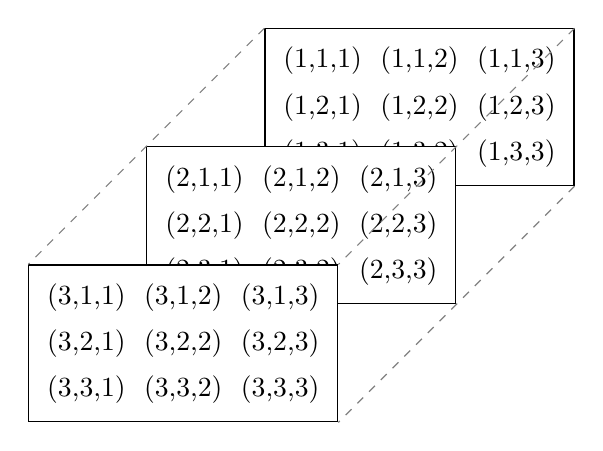
\begin{tikzpicture}
\def\xs{1.5} %shift in x direction
\def\ys{1.5} %shift in y direction
\def\nm{3} % number of 2d matrices in the 3d matrix
\foreach \x in {1,2,\nm}
{

\matrix [draw, % for the rectangle border
         fill=white, % so that it is not transparent
         ampersand replacement=\&] %see explanation
(mm\x)%give the matrix a name
at(-\x * \xs, -\x * \ys) %shift the matrix
{
    \node {(\x,1,1)}; \& \node {(\x,1,2)}; \& \node {(\x,1,3)}; \\
    \node {(\x,2,1)}; \& \node {(\x,2,2)}; \& \node {(\x,2,3)};\\
    \node {(\x,3,1)}; \& \node {(\x,3,2)}; \& \node {(\x,3,3)};\\
};
}

\draw [dashed,gray](mm1.north west) -- (mm\nm.north west);
\draw [dashed,gray](mm1.north east) -- (mm\nm.north east);
\draw [dashed,gray](mm1.south east) -- (mm\nm.south east);
\end{tikzpicture}
\caption{RGB image with 9 pixels  represented as a 3-dimensional matrix}
\label{fig:image_matrix}
\end{figure}

\subsection{Gradient}
\label{se:gradient}
A gradient is a generalization of the derivative in multi-variable space and as such, it is represented as a vector. Like the derivative, it represents the slope of the tangent of the graph of the function. Therefore, it points in the direction of the greatest rate of increase of the function. Gradients are widely used in optimization theory as they allow the parameters to shift in a direction which will minimize or maximize a given function. In machine learning, the function that is to be minimized is the loss function, which is defined in further chapters in more detail. Gradient of $f$ is denoted as $\nabla{f}$, where every component of $\nabla{f}$ is a partial derivative of $f$, denoted as $\frac{\partial{f}}{\partial{x}}\vec{e}$. Notice that gradient components are vectors denoted as $\vec{e_i}$. Every vector is written with a horizontal arrow above the letter, for example, vector $a$ is denoted as $\vec{a}$. The gradient for a $n$ dimensional space is defined in the Expression \ref{eq:gradient}.


\begin{equation} \label{eq:gradient}
    \nabla{f}= \frac{\partial{f}}{\partial{x_{1}}}\vec{e_1} + \hdots +        \frac{\partial{f}}{\partial{x_{n}}}\vec{e_n}
\end{equation}

\subsection{Activation functions} \label{se:activation_functions}
Machine learning models use non-linear functions to gain more capacity - expressiveness. The most popular non-linear functions are $sigmoid$, $tanh$ and $relu$. All non-linear functions have to have easy to compute gradients, as they are computed on parameters in order to reduce loss as explained above. 
\begin{equation} \label{eq:sigmoid}
    sigmoid(x) = \frac{1}{1 + e^{-x}}
\end{equation}

\begin{equation} \label{eq:tanh}
    tanh(x) = \frac{1 - e^{-2x}}{1 + e^{-2}}
\end{equation}

\begin{equation} \label{eq:relu}
    relu(x) = max(0, x)
\end{equation}

The order of non-linear functions is given in order of their discoveries. Today relu is used the most since it solves the problem of vanishing gradients (Section \ref{se:vanishing_gradient} for a detailed explanation of vanishing gradients) for very deep neural networks.

\begin{figure}
    \begin{subfigure}[b]{0.32\textwidth}
        \centering
        \resizebox{\linewidth}{!}{
            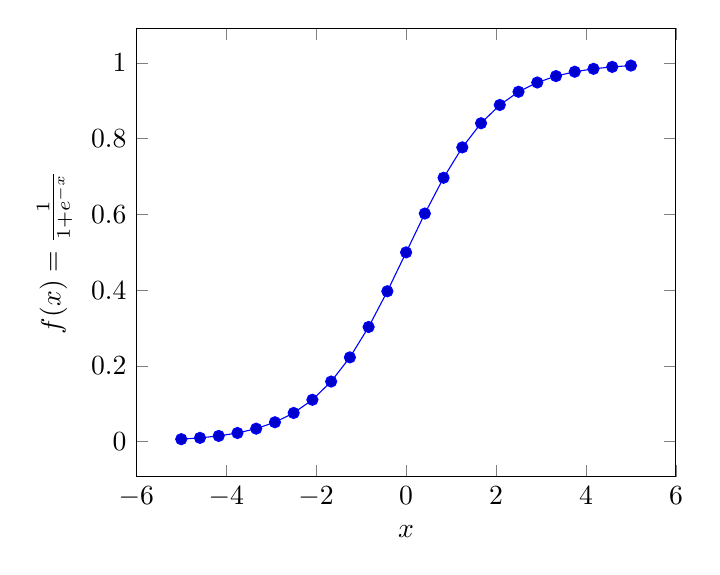
\begin{tikzpicture}
              \begin{axis}[ 
                  mark=none,
                xlabel=$x$,
                ylabel={$f(x) = \frac{1}{1 + e^{-x}}$}
                ] 
                \addplot {1 /(1 + e^-x)}; 
              \end{axis}
            \end{tikzpicture}
        }
        \caption{$simgoid$}
        \label{fig:sigmoid}
    \end{subfigure}
    \begin{subfigure}[b]{0.32\textwidth}
    \centering
        \resizebox{\linewidth}{!}{
            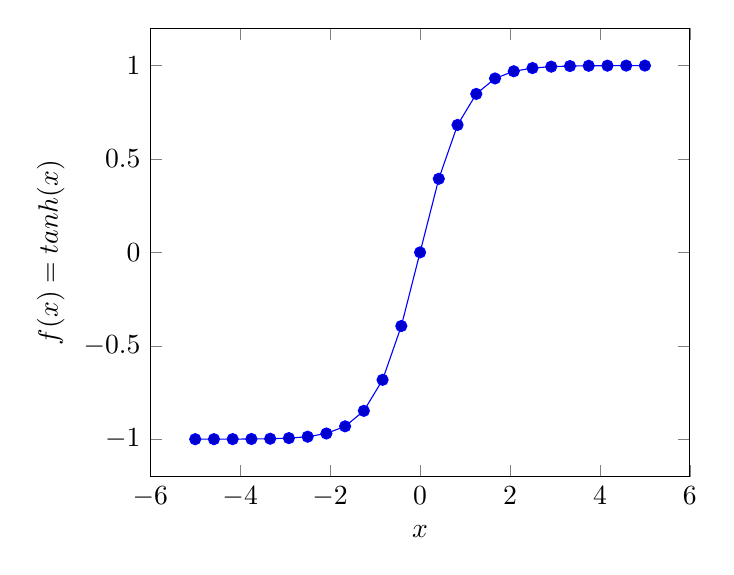
\begin{tikzpicture}
              \begin{axis}[ 
                  mark=none,
                xlabel=$x$,
                ylabel={$f(x) = tanh(x)$}
                ] 
                \addplot {tanh(x)}; 
              \end{axis}
            \end{tikzpicture}
        }
        \caption{$tanh$}   
        \label{fig:tanh}
    \end{subfigure}
    \begin{subfigure}[b]{0.32\textwidth}
        \centering
        \resizebox{\linewidth}{!}{
            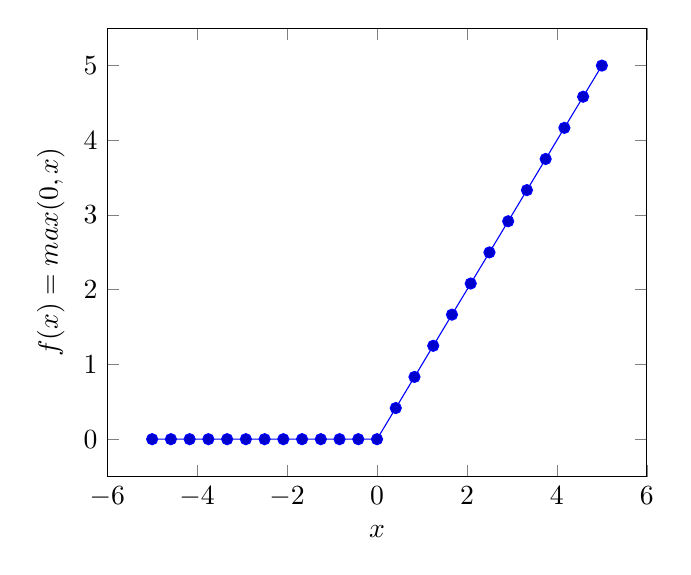
\begin{tikzpicture}
              \begin{axis}[
                  mark=none,
                xlabel=$x$,
                ylabel={$f(x) = max(0, x)$}
                ] 
                \addplot {max(0,x)}; 
              \end{axis}
            \end{tikzpicture}
        }
        \caption{$relu$}
        \label{fig:relu}
    \end{subfigure}
\caption{Non-linear activation functions} 
\label{fig:subfig1.a.4}
\end{figure}

\subsection{Metrics}
\label{se:metrics}
In order to compare different models a set of metrics is employed. Accuracy which gives the accuracy of a model, it is often used on balanced datasets (Expression \ref{eq:accuracy}). The problem with unbalanced datasets can be easily explained with a short example. Imagine having $2$ classes $K=\{dog,cat\}$ and there are a total of $100$ images in the dataset, of which only $2$ are dogs. The model, if optimized for accuracy might say the whole dataset is composed of cats which will yield an accuracy of $98\%$. To solve the previous problem, additional metrics were introduced for the task of classification; precision (Expression \ref{eq:precision}), recall (Expression \ref{eq:recall}) and F1 score (Expression \ref{eq:f1score}). Precision - positive predictive value - is defined as a fraction of retrieved instances that are relevant. Recall - sensitivity - is a fraction of relevant instances that are retrieved. In order to represent the performance of a model as a single variable F1 score was introduced, it represents a harmonic mean of recall and precision.
\begin{equation} \label{eq:accuracy}
    Accuracy = \frac{tp + tn}{tp + tn + fp + fn}
\end{equation}

\begin{equation} \label{eq:precision}
    Precision = \frac{tp}{tp + fp}
\end{equation}

\begin{equation} \label{eq:recall}
    Recall = \frac{tp}{tp + fn}
\end{equation}

\begin{equation} \label{eq:f1score}
    F1 score = 2 * \frac{precision * recall}{precision + recall}
\end{equation}



Classification results are often represented as a confusion matrix, also known as an error matrix.  It is a  way to visualise the performance of a classification model - classifier. To build the classification matrix, conditions of the experiment must be labeled as positive or negative. Using the cats and dogs example from before and making the cats a positive and dogs a negative class creates a $2 \times 2$ matrix of actual and predicted values as shown in Table \ref{tb:confusion_matrix}.

\begin{table}
\centering
\caption{Confusion matrix}
\label{tb:confusion_matrix}
\begin{tabular}{|c|c|c|}
\hline 
 & \textbf{prediciton} positive & \textbf{prediction} negative \\ 
\hline 
\textbf{actual} positive & True Positive (TP) & False Negative (FN) \\ 
\hline 
\textbf{actual} negative & False Positive (FP) & True Negative (TN) \\ 
\hline 
\end{tabular}
\end{table}

\subsection{Data} \label{se:data}
The input data of the machine learning algorithm is labelled as $D$, and it consists of $X$ and $y_{t}$, where $X$ is one input data point (an image in our case) and $y_{t}$ is the true label of that image - species' name. Written formally the whole input dataset is represented as $D = \{{X}^{\,i},y^{\,i}\}^{N}_{i=1}$, where $i$ is the $i$-th data point and $N$ is the number of data points. The predicted value for an input data point $X$ is labelled as $y_{p}$.

The input data set is usually split into two datasets - called the \textit{training} and the \textit{test} dataset. The training dataset is used to optimize the model's parameters while the test data is used to evaluate the model's performance on previously unseen data - the goal of machine learning is the create models that work well on previously unseen data. Sometimes the training dataset is split further into training and \textit{validation} where the validation dataset is used to tune the models \textit{hyperparameters}. Hyperparameters are parameters that do not belong to the model but  effect the model's performance. The depth of the neural network is a type of hyperparameter and will be discussed in later chapters in more detail.


\section{Machine learning}
\label{se:machine_learning}

As said in the Chapter \ref{se:introduction} - Introduction, machine learning allows computers the ability to learn. Giving data to a machine learning algorithm - model - allows it to find patterns within the dataset. The function that maps the input $X$ to $y_p$ is called a \textit{hypothesis} and is denoted as $h$ (Expression \ref{eq:hypotesis}). The hypothesis $h(X ; \vec{\theta})$ is parametrized with $\vec{\theta}$ - model's parameters.

\begin{equation} \label{eq:hypotesis}
    h(X ; \vec{\theta}) : X \to y
\end{equation}


The model is defined as a set of hypothesises $H$, $h \in H$. Machine learning can be defined as the search of the best hypothesis $h$ from the hypothesis space $H$ - typical optimization problem. The algorithm tries to minimize the empirical error function $E(h|D)$ - loss function. The error indicates the accuracy of the hypothesis and is called empirical because it is computed on $D$. Therefore, every machine learning algorithm is defined with the model (Expression \ref{eq:model}), error function (Expression \ref{eq:error_function}) and the optimization method (Expression \ref{eq:optimization_function}).

\begin{equation} \label{eq:model}
    H = \{ h(X ; \vec{\theta}) \}_{\theta}
\end{equation}

\begin{equation} \label{eq:error_function}
    E(h|D) =  \frac{1}{N} \displaystyle\sum_{i=1}^{N} I\{h(X^{\,i}) \neq y^{i}\}
\end{equation}

\begin{equation} \label{eq:optimization_function}
    \theta^{*} = argmin_{\theta} E(\theta | D)
\end{equation}


Machine learning algorithms are divided into groups depending on the task, the groups are classification, clustering, and regression. Each can be represented as a result of $h(X ; \vec{\theta})$. Classification hypothesis takes the input $X$ and returns a class $k$, an example of this method would be image classification. Regression hypothesis takes the input $X$ and returns a number, for example predicting house prices.

\begin{equation} \label{eq:regression_def}
    Regression - h(X ; \vec{\theta}) : X \to y, y \in \mathbb{R}
\end{equation}

\begin{equation} \label{eq:classification_def}
    Classification  - h(X ; \vec{\theta}) : X \to y, y \in K = \{k_{0}, ..., k_{n}\}
\end{equation}

In this chapter, it was mentioned that machine learning algorithms are trained by minimizing the empirical loss, and in the Section \ref{se:data} the idea of having a training and test set was introduced. The goal of the machine learning model is to have good generalization - the ability to perform well on never before seen data. The training set $X_{train}$ is used by the optimization algorithm to tune the model's parameters, while the test set $X_{test}$ is used to evaluate the generalization performance of the model. If the optimization algorithm does not know when to stop it can learn the whole training set and be able to predict every value, this is called overfitting and it is to be avoided. When the model overfits, it learns to predict based on the data points in $X_{train}$ instead of the learning the underlying patterns in $X_{train}$, which in turn leads to poor generalization performance. This is commonly seen in models with high capacity. On the other hand, if the model has low capacity, it will under-perform - work below its potential. That is referred to as underfitting. To goal is to find the optimal performance of the model - between underfitting and overfitting. This behavior can be seen in Figure \ref{fig:overfitting}. The x-axis shows the number of training epochs - each epoch increases the capacity of the model. The training error $E_{train}$ is falling asymptotically towards zero while the generalization performance start to fall certain a point (50 epochs). The ideal situation for the model is to stop the training when the model starts to overfit, which is not that easy as we will see in the future chapters.


\begin{figure}
  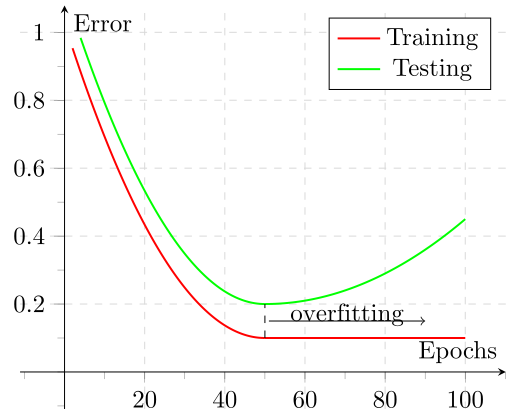
\includegraphics[scale=0.43]{figures/overfitting.png}
  \centering
  \caption{Performance of a model by the number of epochs using training and test set}
  \label{fig:overfitting}
\end{figure}



One way to combat overfitting is by early stopping during training. Another, more popular way is to use regularization. Regularization is a technique for increasing the generalization performance of the model by penalizing high parameter values or reducing the complexity of the model. There is a broad set of regularization techniques used in machine learning models. Some of the most popular for artificial neural networks are called Dropout \citep{srivastava_dropout:_2014} and data augmentation, both of which will be explained in more detail in future chapters (Sections \ref{se:dropout} and \ref{se:data_augmentation}). Regularization techniques usually add additional components to the loss function in order to prevent the model from learning to map $X_{train}$ to $y_{train}$ directly.


\subsection{Supervised and unsupervised learning}
For the model to be trained it needs data $D$ which is defined as $\{{X}^{\,i},y^{\,i}\}^{N}_{i=1}$. Unfortunately, $y$ is not always available. In such cases, the model can still use only $X$ to infer and that is called unsupervised learning. When the model uses both the data points $X$ and labels $y$ it is called supervised learning. Classification and regression are both cases of supervised learning. Cluster analysis or more commonly called clustering is a type of unsupervised learning. In clustering, the model tries to group a set of objects in such a way that objects in the same group are more similar based on a certain metric. The groups are called clusters, hence the name clustering. Some algorithms need the number of clusters to be predefined, while others discern it by themselves. As the purpose of the task is by itself classification, in following chapters supervised learning methods will be explained in more detail.

\subsection{Artificial neural network (ANN)}
One of the most interesting models in machine learning, with a diverse set of variations, are artificial neural networks (ANN). The computational model based on mathematics for neural networks was first introduced in 1943 by Warren McCulloch and Walter Pitts \citep{mcculloch_logical_1943}  called threshold logic. Later on, in 1951 an influential paper was published by S. C. Kleene on linking neural networks to finite state automata \citep{kleene_representation_1951}. Artificial neural networks are based on a large collection of small computational unites called neurons (Figure  \ref{fig:ann_neuron}). The architecture was inspired by axons (Figure \ref{fig:neuron}) from our brains. The idea is that even though a single neuron does not have the capacity to express complicated levels of abstractions - neurons together can. Neurons are connected in order to transfer signals. If a neuron receives a strong enough signal it becomes activated and propagates the received signal toward his output. Just propagating the signal would not be of benefit, as the signal would not transform while passing trough the network, therefore non-linear activation functions, as explained in Section \ref{se:activation_functions}, are added to each output of a neuron.

\begin{figure}
  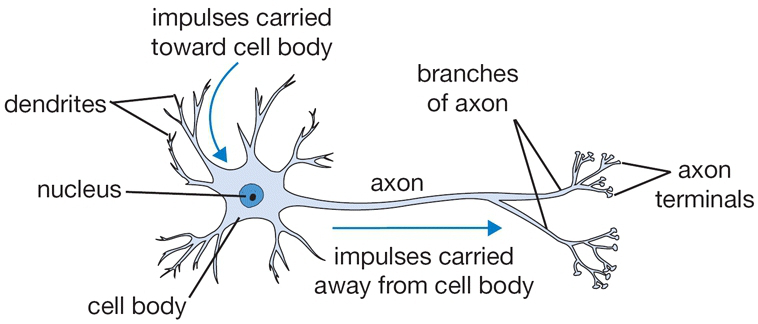
\includegraphics[width=\linewidth]{figures/axon.png}
  \caption{Neuron cell in a brain}
  \label{fig:neuron}
\end{figure}

\begin{figure}
  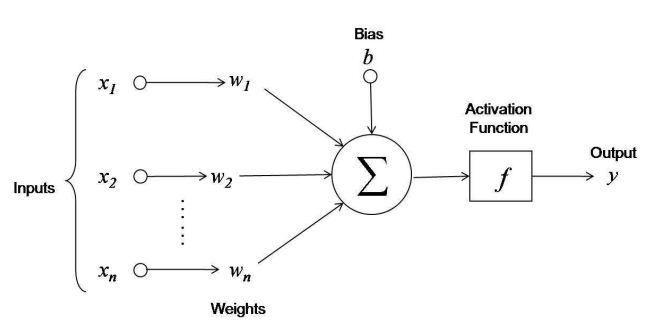
\includegraphics[width=\linewidth]{figures/neuron.jpg}
  \caption{Artificial neuron cell}
  \label{fig:ann_neuron}
\end{figure}

One of the most popular ANN architectures are feed-forward networks (FFN), consisting of fully-connected layers or sometimes also referred to as dense layers. They are called feed-forward because the data $X$ enters at one side of the network (the input layer) and exits at the other end (output layer). Neurons are grouped into layers, and layers make an artificial neural network. The first layer is called an input layer, the last layer is called the output layer and every layer in between is a hidden layer. The network is called fully-connected because each neuron in the hidden and output layers are connected with ever neuron of the previous layer as seen in Figure \ref{fig:ann}.
Each neuron consists of connections, a bias and an activation function. Each connection has a weight that singles the importance of the connection to the neuron. To get the net output of the neuron we multiply the input vector $\vec{x}$ with the weight vector $\vec{w}$. As the bias (commonly denoted with $w_0$ or $b$), does not have an input of its own, we assigned $x_0$ to 1 to be able to do vector multiplication (Expression \ref{eq:neuron_net_output}). To get the final output $y$ of the neuron, the activation function $f$ is applied to the $net$ output, as shown in the Expression \ref{eq:neuron_output}). The computational model of the artificial neuron can be seen in the Figure \ref{fig:ann_neuron}.

\begin{equation}
    \label{eq:neuron_net_output}
    net = 1*w_0 + w_1*x_1 + ... + w_n*x_n = \vec{x} * \vec{w}
\end{equation}

\begin{equation}
    \label{eq:neuron_output}
    y = f(net) = f(\vec{x}*\vec{w})
\end{equation}

\begin{figure}
  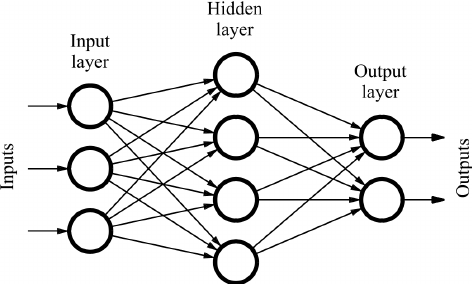
\includegraphics[width=\linewidth]{figures/ann.png}
  \caption{Feed-forward neural network}
  \label{fig:ann}
\end{figure}


Artificial neuron networks have the ability to adjust their capacity to the task. Adjusting the number of neurons in a single layer, the number of hidden layers or the type of activation function used in each neuron affects the capacity of the ANN. Such flexibility also leads to a broad number of architectures, and there is no clear way to determine which one is best for the task. It is often left to the user to test a broad variety of architectures. Figure \ref{fig:ann} shows that the number of neurons in the input layer matches the input size, this is true also for the output layer. Therefore, when designing an ANN the size of input and output layers are determined by the task and the number of hidden layers by the user.


\section{Deep learning}
\label{se:deep_learning}
Deep learning is a class - subset - of machine learning algorithms. Even though deep learning may be connected to using "deep" neural networks - neural networks with many layers - it was created as a subset of machine learning that promised the automation of feature extraction task by using unsupervised learning. Unsupervised feature extraction and feature representation are done through a cascade of many non-linear layers, each of which contains artificial neurons. 

Visual recognition is one of the fields that is most affected by improvements in deep learning \citep{krizhevsky_imagenet_2012, simonyan_very_2014, szegedy_going_2015, he_deep_2016}. It's difficult and time-consuming to build hand-crafted features for each visual recognition problem. Deep learning allows the user to use raw images with minimal preprocessing - making it applicable with ease to almost any task.

Deep learning algorithms consist of enormous numbers of parameters (hundreds of millions), therefore training them is computationally expensive. Recent breakthroughs in deep learning were driven by advances in hardware - graphics processing unit (GPUs). GPUs are made of a lot of processor unites, making them ideal for highly concurrent tasks. Neural networks are easily trained concurrently because of their composite structure and a special training algorithm called Stochastic backpropagation (discussed in detail in Section \ref{se:backprop}), commonly referred to as backprop.

\subsection{Convolutional neural network (CNN /  ConvNet)}
The convolutional neural network is a type of feed-forward network that was inspired by the organization of animal's visual cortex. They are used in recommender systems, natural language processing, and image recognition. The architecture was inspired by the works of Huble and Wiesel in 1950s and 60s \citep{hubel_receptive_1968}. Their work showed that animal's visual cortex contains neurons that individually respond to small regions in the visual field. As well as,  that neighbourhood neurons had similar receptive fields.

The necognitron was introduced in the 1980s by Kunihiko Fukushima \citep{fukushima_neocognitron:_1982, eckmiller_hierarchical_1989} and served as an inspiration for today's modern convolutional neural network architecture. The necognitron is a hierarchical multi-layered artificial neuron network. It was used for handwritten character recognition, which belongs in the domain of image recognition.

\begin{figure}
  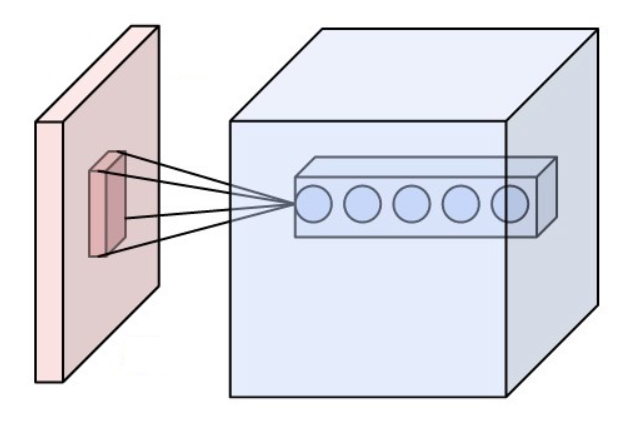
\includegraphics[scale=0.5]{figures/conv.png}
  \centering
  \caption{3-dimensional structure of a convolutional filter (on the left painted in pink is the input - image - and the blue rectangle with circles is a filter)}
  \label{fig:conv}
\end{figure}

Today's modern convolutional neural network architectures, such as: AlexNet, VGG, Inception and ResNet \citep{krizhevsky_imagenet_2012, simonyan_very_2014, szegedy_going_2015, he_deep_2016} are made mostly of convolution and pooling layers. These architectures have an enormous number of parameters and are trained on powerful GPUs or clusters of servers over a period of days, sometimes even weeks.

The convolution layer is a building block of modern CNNs. The layer's parameters consist of a set of kernels (filters). Each filter has a small receptive field but extends through the whole depth of the input. During the forward pass of the input through the network, each filter is convolved across the width and height of the input volume. Each time the filter moves to neighbourhood pixels it creates an output pixel (shown in Figures \ref{fig:conv} and \ref{fig:conv1}). Each convolution layer consists of multiple filters, each specialized (because of model optimization - training) to detect different features in the input. Filters will detect diagonal edges, top edges, corners and other different building blocks of images. Each filter will use the features of the previous layer to create more abstract features. For example, a filter in the first layer might capture edges, while filters in deeper layers may use the edge filters to create corner and circle detectors (shown in detail in Figure \ref{fig:filter}) \citep{simonyan_very_2014}.


\begin{figure}
  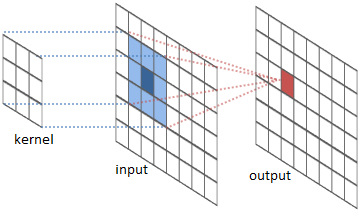
\includegraphics{figures/conv1.png}
  \centering
  \caption{A $3 \times 3$ kernel (filter) convolving and input to generate an output}
  \label{fig:conv1}
\end{figure}

\begin{figure}
  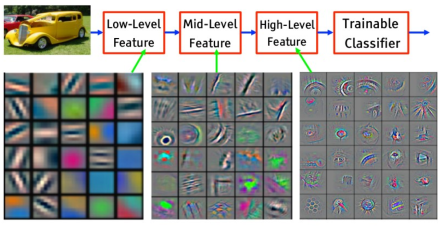
\includegraphics[scale=1.4]{figures/filter.png}
  \centering
  \caption{Representation of filters throughout the CNN}
  \label{fig:filter}
\end{figure}

The second core layer of almost every modern CNN is the pooling layer. It, in contrast to the convolution layer, does not have any parameters. The pooling layer takes the input and reduces its dimension. CNNs use max pooling, which maps the input into a reduced output by taking only the max values in the mapping (showed in Figure \ref{fig:pool}). Use of pooling layer is a heated topic in today's CNN architectures, unfortunately, hardware cannot keep up with the depth of the modern architectures without the use of pooling layers.

\begin{figure}
  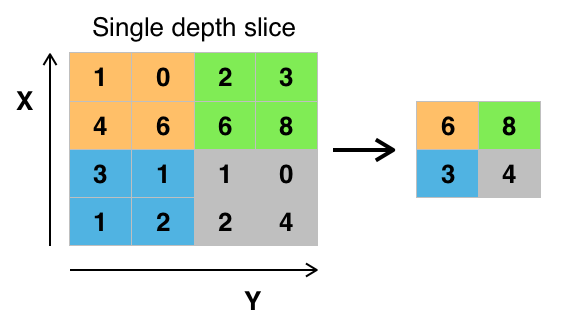
\includegraphics[scale=0.6]{figures/pool.png}
  \centering
  \caption{Max pooling a $4\times4$ input to $2\times2$}
  \label{fig:pool}
\end{figure}

The typical structure in a CNN is one or more convolution layers followed by a max pool layer, and that is repeated multiple times to increase the capacity of the model. The most common dimension of convolution filters is $3\times3$, made popular by the huge success of VGG \citep{simonyan_very_2014} CNN architecture. The typical CNN is shown in Figure \ref{fig:cnn}.

\begin{figure}
  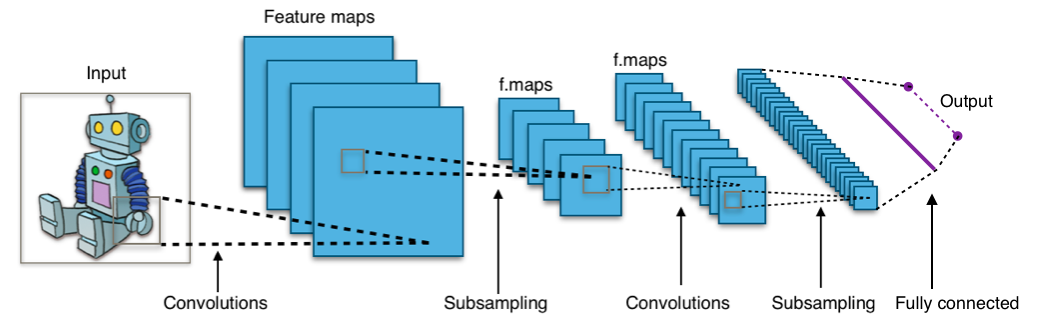
\includegraphics[scale=0.43]{figures/cnn.png}
  \centering
  \caption{Typical modern CNN}
  \label{fig:cnn}
\end{figure}

\subsection{Dropout} \label{se:dropout}

One of the most important techniques in machine learning is regularization (Section \ref{se:machine_learning}). One way to regularize neural networks is with the Dropout technique that was introduced in 2014 \citep{srivastava_dropout:_2014}. Dropout "drops" (removes) a percent of neurons on every forward pass (Figure \ref{fig:dropout}). The network cannot be sure that the same neurons will always be active and, as a result, must not rely on every neuron, therefore increasing the robustness of the model together with its generalization performance. As in every forward pass, the network has a different set of neurons, this technique can be seen as using multiple variations of the same network on the same problem.

\begin{figure}
  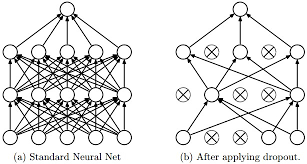
\includegraphics[scale=0.91]{figures/dropout.png}
  \centering
  \caption{An example of the Dropout technique}
  \label{fig:dropout}
\end{figure}

\subsection{Data augmentation}  \label{se:data_augmentation}

Another popular regularization technique is called data augmentation. The model usually trains in tens or even hundreds of epochs - a signal epoch is when the training algorithm uses every data point in $X_{train}$ (one pass over $X_{train}$). Reusing the same data points can lead to overfitting. One approach to preventing that is to augment $X_{train}$ on every epoch. Usually the data is augmented with rotation, mirroring, cropping, blurring (all these effects can be seen in Figures \ref{fig:data_augmentation_figure} and \ref{fig:data_augmentation}). Both dropout and data augmentation are used in almost every state-of-the-art CNN model today. There are some exceptions due to a new technique called batch normalization \citep{ioffe_batch_2015}.

\begin{figure}
  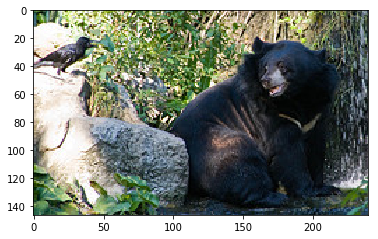
\includegraphics[scale=0.7]{figures/data_augmentation.png}
  \centering
  \caption{An example of the original - unprocessed - image in $X_{train}$}
  \label{fig:data_augmentation_figure}
\end{figure}

\begin{figure}
  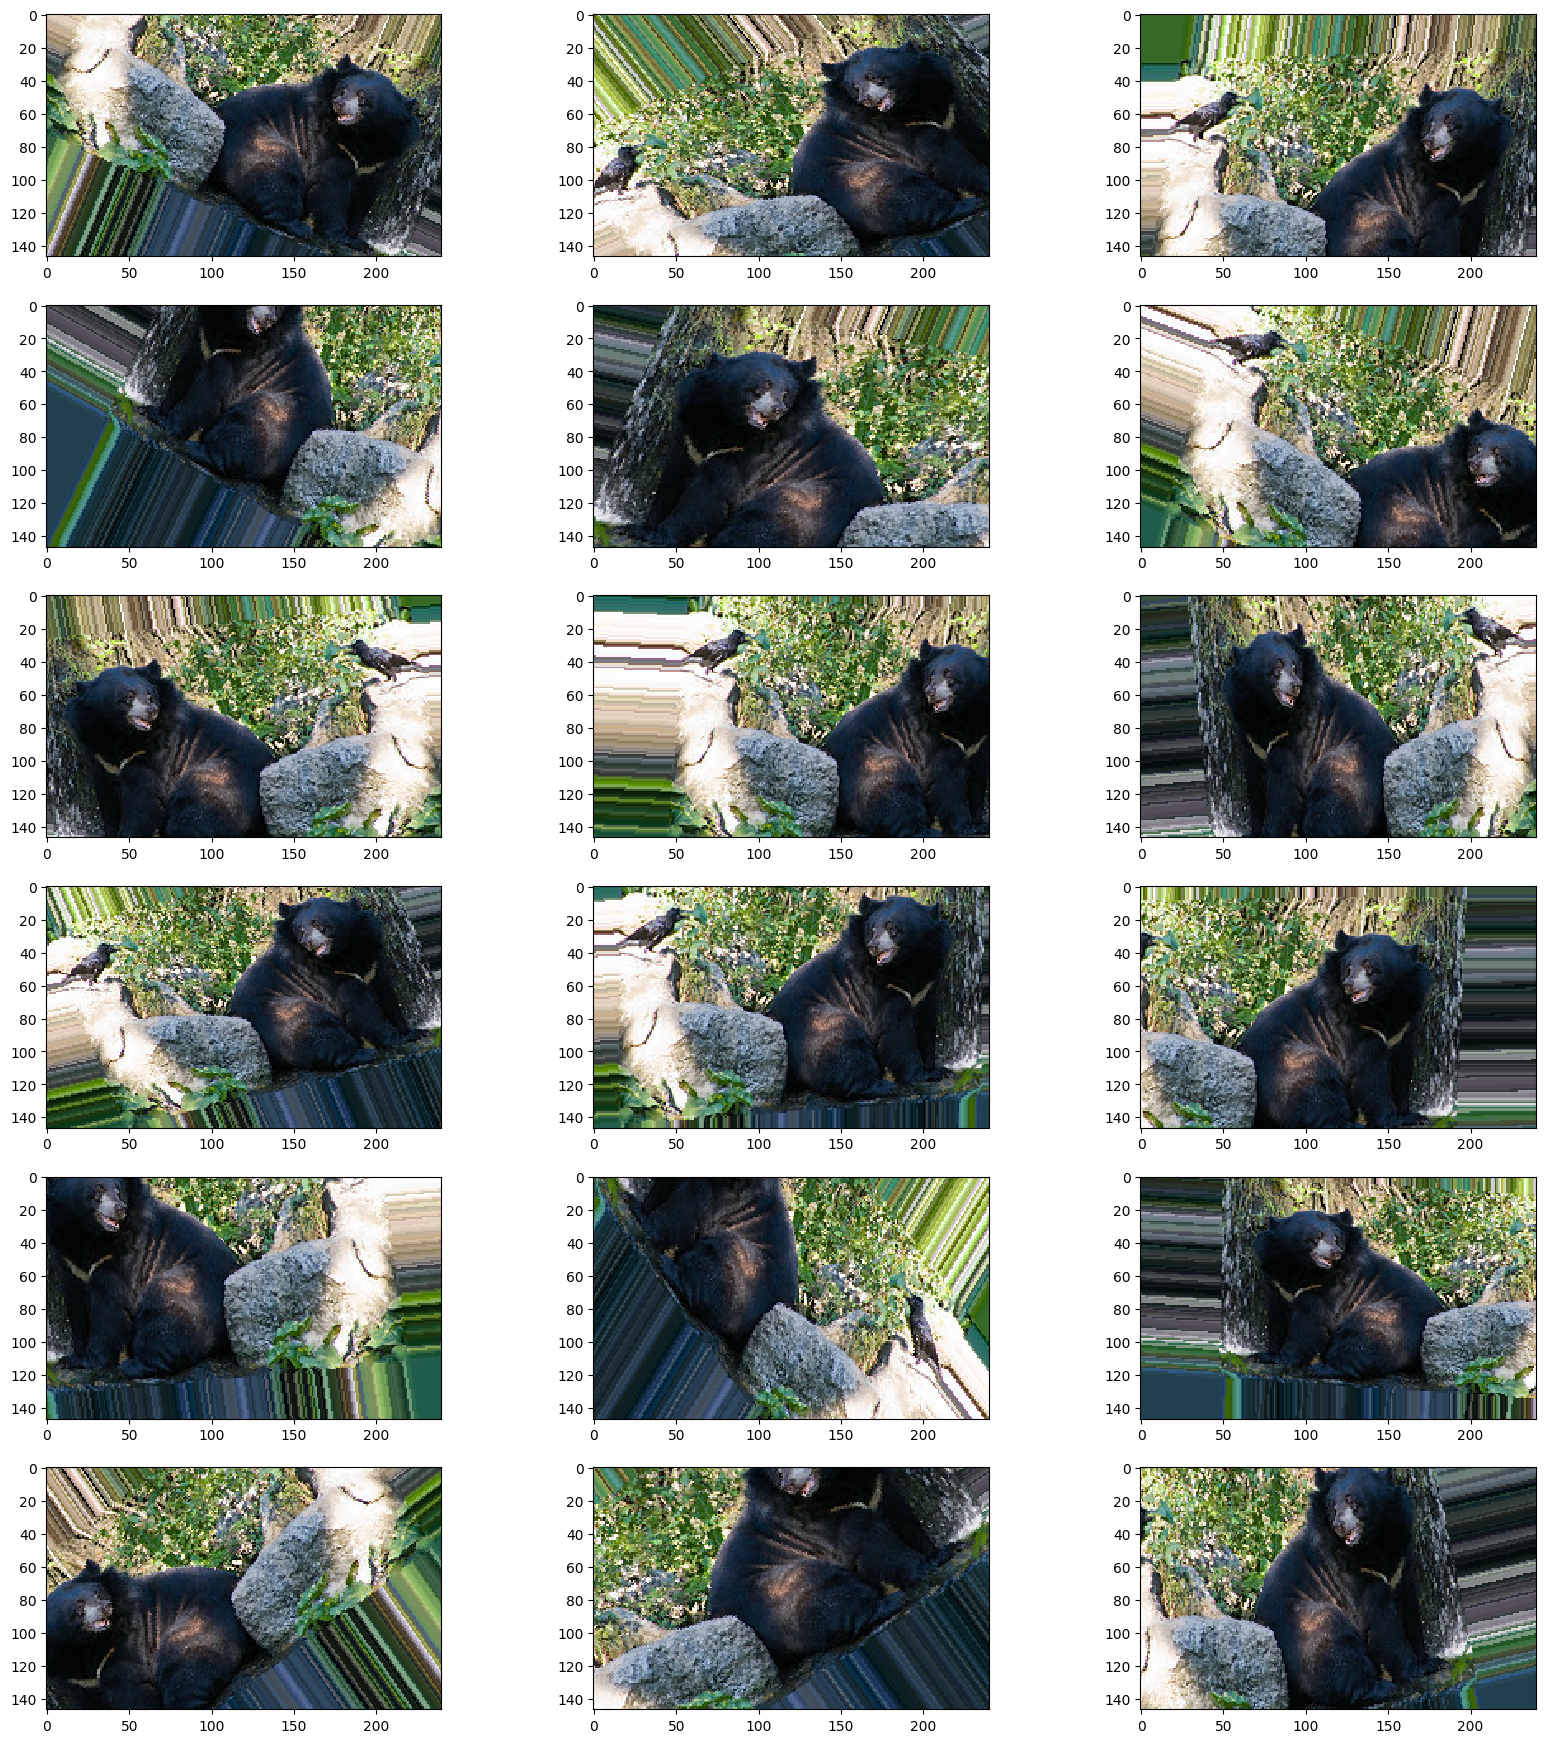
\includegraphics[scale=0.35]{figures/da1.png}
  \centering
  \caption{Example of data augmented images based on the original Figure \ref{fig:data_augmentation_figure}}
  \label{fig:data_augmentation}
\end{figure}

\subsection{Backpropagation} \label{se:backprop}

To be able to train a convolutional neural network on huge datasets, an algorithm is needed that is able to train the model with a subset of $X_{train}$. Fitting the whole $X_{train}$ in the GPU memory is not possible for datasets of serious size. Also, the algorithm should be highly concurrent in order to use the structure of the neural network to its advantage. The backward propagation of errors or more commonly called Backpropagation (backprop) used together with gradient descent is the most popular method for training (most) neural networks.

\subsubsection{Gradient descent}

Gradient descent is an iterative optimization algorithm. It uses the gradient (Section \ref{se:gradient}) of a function to find a point on a domain that minimises or maximises the function's value. Gradient descent does not guarantee to find the global maximum or minimum (Figure \ref{fig:local_and_global_function_values}). There have been several variations of the gradient descent algorithm that deal with the algorithm being stuck in local maximum or minimum, the most famous and most widely used for deep learning is Adam \citep{kingma_adam:_2014}.

\begin{figure}
  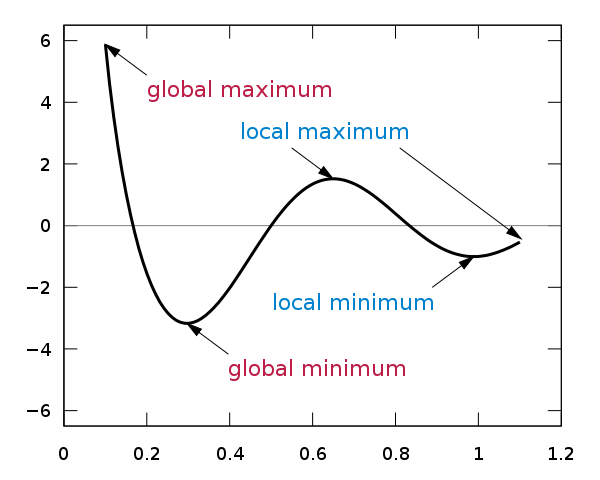
\includegraphics[scale=0.5]{figures/local_global_maxima_minima.png}
  \centering
  \caption{An example of local and global maximum and minimum in a function}
  \label{fig:local_and_global_function_values}
\end{figure}

\begin{equation} 
\label{eq:gradient_descent}
    x_{n+1} = x_n - \eta * \nabla{f(x_n)}
\end{equation}

Gradient descent uses the gradient of a function to move in a way that minimises or maximises the given function (Expression \ref{eq:gradient_descent}). The amount that is used to move the data point - called the step ($\eta$) - is crucial for the convergence of the algorithm. If the step is too big the algorithm might diverge or get stuck into a local minimum or maximum, while if the step is too small the algorithm might take too long to converge. Gradient descent, like other optimization algorithms, needs to have its parameters properly initialised to achieve good results.

\begin{figure}
  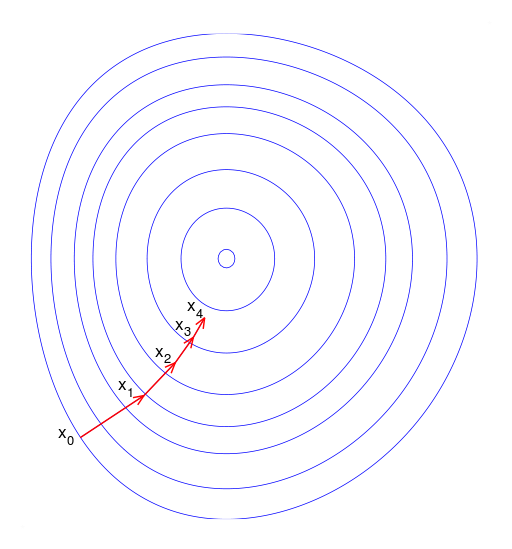
\includegraphics[scale=0.5]{figures/gradient_descent.png}
  \centering
  \caption{An example of gradient descent converging to the global minimum in a 2-dimensional space (function with two variables)}
  \label{fig:local_and_global_function_values}
\end{figure}

\subsubsection{Stochastic gradient descent}
\label{se:stochastic_gd}

The main disadvantage of the Gradient descent algorithm (Expression \ref{eq:gradient_descent}) is the need to calculate the gradient on all the dataset, to be able to update the parameter. The gradient has to be calculated on the whole $X_{train}$. An improvement on the basic Gradient descent is the Stochastic gradient descent (SGD) \citep{bottou-98x}. It updates the gradient by sampling the dataset in mini-batches, usually the size 64, 128 or 256 data points (depending on GPU memory limitations). After every epoch, the whole training dataset $X_{train}$ is shuffled so that different mini-batches will be sampled in the next epoch. The rule of thumb is if you can increase the size of mini-batch - do it. The more data points are in the mini-batch, the more precise is the gradient approximation, also the model trains faster.

\subsubsection{Optimization target}

The goal of the Gradient descent algorithm is to minimise or maximise a function. In deep learning, when training the model, the goal is to minimise the loss function $E(h|D)$ by computing its gradient. In classification (Expression \ref{eq:classification_def}) the goal is for the predicted class $y_p$ to match the true class $y_t$. Neural networks for classification usually have a softmax layer as their last layer. Softmax (Expression \ref{eq:softmax}) is a normalization exponential function, which transforms neural network's outputs to probabilities for every class. The sum of the softmax values for all classes is equal to one.  

\begin{equation}
\label{eq:softmax}
    softmax(\vec{z})_j = \frac{e^{z_j}}{\displaystyle\sum_{k=1}^{K} e^{z}_k} \quad \text{for} \quad j = 1, ..., K
\end{equation} 

For the task of classification, the softmax function is the final layer - the output. Using this information allows us to compute the loss function. The loss of a softmax function is called cross-entropy loss and is computed with negative log likelihood (Expression \ref{eq:cross_entropy_loss}).

\begin{equation}
\label{eq:cross_entropy_loss}
    L(y_t, y_p) = - \displaystyle\sum_{d=1}^{D} \sum_{k=1}^{K} y^i_t * log(y^i_p) 
\end{equation}

To use the cross-entropy loss in the Backpropagation we have to calculate its gradient. The gradient for cross-entropy loss is shown in the Expression \ref{eq:cross_entropy_graidnet}).

\begin{equation}
\label{eq:cross_entropy_graidnet}
 \nabla{L} = \vec{y_t} - \vec{y_p}
\end{equation}

\subsection{Vanishing gradient}
\label{se:vanishing_gradient}

On of the problems with using Backpropagation is the propagation of loss gradients in the neural networks. As the neural network is composed of smaller unites called neurons, its output is also a function composed of linear combinations and non-linear activation functions of previous layers. The Backpropagation algorithm calculates the gradient losses from the output to the front layers of the neural network - hence the name Backpropagation. The deeper the network, the more information is lost due to gradient decay - low gradient values. The vanished gradient means that the network is not efficiently training and leads to poor performance. One way to combat that is to use special activation functions \citep{clevert_fast_2015, xu_empirical_2015, he_delving_2015} or special architectures \citep{he_deep_2016} that deal with this problem. 


\subsection{Batch normalization}
\label{se:batch_norm}

Normalizing input data before it enters the machine learning algorithm usually increases the performance of the algorithm. It is easier for the model to learn its task when all of its inputs will be in a certain range. Input normalization in CNNs that use images for input will not yield significant performance improvements because the input for images are normalized by nature in the range of $0$ to $255$ RGB values (Section \ref{se:data}). 

The second problem is the modularity of neural networks. Each layer feeds its outputs into the inputs of the next layer - making any input normalization futile. To combat this a new solution in a form of normalization layer has been introduced in 2015 called batch normalization \citep{ioffe_batch_2015}. It normalizes the data for the whole minibatch that is used in the forward pass of the backpropagation algorithm (Section \ref{se:backprop}). As the authors have shown, using batch normalization improves generalization, in some cases removes the need for Dropout (Section \ref{se:dropout}) and makes the neural network more robust to initial hyperparameter initialization.

\chapter{Model}
\label{se:model}
To make a scalable species classifier that works with specific hardware requirements I had to make a classifier that yields the best performance and could be trained on a GPU with 2GB of RAM in a reasonable time. In this chapter, I introduce my solution based on the convolution neural network architecture ResNet \citep{he_deep_2016}.


\section{Implementation}

There are a plethora of computational frameworks to choose to create a deep learning model; TensorFlow \citep{tensorflow}, Caffe2 \citep{caffe}, pyTroch \citep{pytorch}, Keras \citep{keras}, Theano \citep{theano}, CNTK \citep{cntk} and many more. I have chosen Keras as it has a high-level API for creating neural networks and provides pretrained models (more on this in Section \ref{se:pretrained_parameters}) which were crucial to train a high accuracy model on a weak GPU. Keras allows the user to choose a backend deep learning framework, at the time of writing this thesis there were two options - TensorFlow and Theano. TensorFlow was chosen as it is newer and has gained a lot of popularity in the past couple of months.

\subsection{Keras}
\label{se:keras}

Keras provides a high level of abstraction when creating neural networks, giving the user a framework for rapid iteration and development. A simple example of the high-level API is given below. Using Keras we can create a two-layered feed-forward neural network in just a couple of lines of code. The "create\textunderscore model" function returns a model with two layers the first layer has 32 neurons, the second (also the last) has 10 - this means the classifier has 10 classes (the number of neurons in the last layer should always match the number of classes). The last layer uses the softmax activation function (Expression \ref{eq:softmax} for more details) to get class probabilities. The model also defines to type of gradient descent algorithm (Expression \ref{eq:gradient_descent}) - RMSProp, and the loss function categorical cross entropy (Expression \ref{eq:cross_entropy_loss}). The "train\textunderscore model" function takes the created model and trains it in 10 epochs with a minibatch size of 32 input data points (Section \ref{se:stochastic_gd}).



\begin{lstlisting}[language=Python, caption=Keras' high-level API example]
from keras.layers import Dense

def get_data():
    ...
    return X_train, y_train

def create_model():
    model = Sequential()
    model.add(Dense(32, input_shape=(500,)))
    model.add(Dense(10, activation='softmax'))
    
    model.compile(optimizer='rmsprop',
          loss='categorical_crossentropy',
          metrics=['accuracy'])
          
    return model
    
def train_model(model, X_train, y_train):
    model.fit(X_train, y_train,
      batch_size=32, epochs=10)
        
X_train, y_train = get_data()
model = create_model()
train_model(model, X_train, y_train)

\end{lstlisting}

TensorFlow is the backend engine of Keras, and it, same as Keras, allows the user to write computational graphs in Python. Python is a high-level language that allows the user for rapid development due to its simplicity. All computational graph frameworks mentioned above work blazingly fast, yet they use (mostly) Python to define the computational graph (neural network). The key to fast performance for these frameworks is that they are written and run in C++, but they offer a high-level API in Python. For this to work the API usually has a "compile" function that builds the graph and the "train" or "fit" function which starts the process of training the neural network.

\subsection{Architecture}
\label{se:architecture}

There are a lot high performance CNN architectures \citep{he_deep_2016, simonyan_very_2014, szegedy_going_2015}, they offer different performance levels with varying parameter sizes, as shown in Table \ref{tb:CNN_architecutre_performance}. To classify species on a 2GB GPU I needed a powerful yet small neural network. ResNet and Inception v3 are perfect for the task as they give a competitive performance per parameter number ratio, especially the ResNet-50. Obviously, one can create its own architecture but doing that removes the performance boost of pretrained models, this is explained in more detail in a future Section \ref{se:pretrained_parameters}. The final architecture consisted of a base pretrained model with a feed-forward neural network on top of it. Two main candidates for the base network were the ResNet-50 and Inception v3 CNN architectures. As shown in Section \ref{se:resnet_vs_inception}, the ResNet-50 architecture gave better results on this particular task and was chosen to be the base neural network for the model.

\begin{table}
\centering
\caption{CNN architecture performance comparison on ImageNet dataset ($error = 1 - accuracy$)}
\label{tb:CNN_architecutre_performance}
\begin{tabular}{ccc}
\hline 
Network    & Top-1 error & Top-5 error \\  \hline
ResNet-18 & 30.24 & 10.92 \\
ResNet-34 & 26.70 & 8.58 \\ 
ResNet-50 & 23.85 & 7.13 \\ 
ResNet-101 & 22.63 & 6.44 \\ 
ResNet-152 & 21.69 & 5.94 \\  \hline
Inception v3 & 22.55 & 6.44 \\
\hline 
\end{tabular} 
\end{table}

\subsection{ResNet} 
\label{se:resnet_architecture}

ResNet's performance comes from a unique way in which it builds layers. ResNet is short for the residual neural network - residual is the input of a layer that is being summed to the layers output, giving input information a path for input to circumvent the layer's transformation. This method allows for very deep neural networks to converge when trained. The residual can pass one layer or more, the architecture in the paper uses two convolution layers between each residual (Figures \ref{fig:residual_layer} and \ref{fig:vgg_resnet_comparison}).

\begin{figure}
  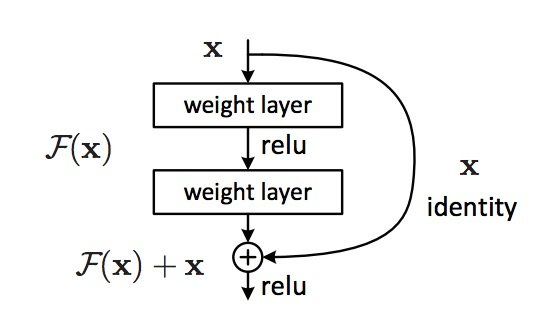
\includegraphics[scale=0.55]{figures/resiudal_layer.jpg}
  \centering
  \caption{The residual layer (module) - the core building block of the ResNet}
  \label{fig:residual_layer}
\end{figure}

Figure \ref{fig:vgg_resnet_comparison} shows a direct comparison between VGG \citep{simonyan_very_2014} and ResNet architectures. One of the main benefits of using ResNet is a lower memory consumption on the GPU because of the lack of fully-connected (dense) layers at the end of the network. The fully-connected layers contain the most parameters, and removing them increases the number of convolution layers while lowering the number of parameters.

\begin{figure}
  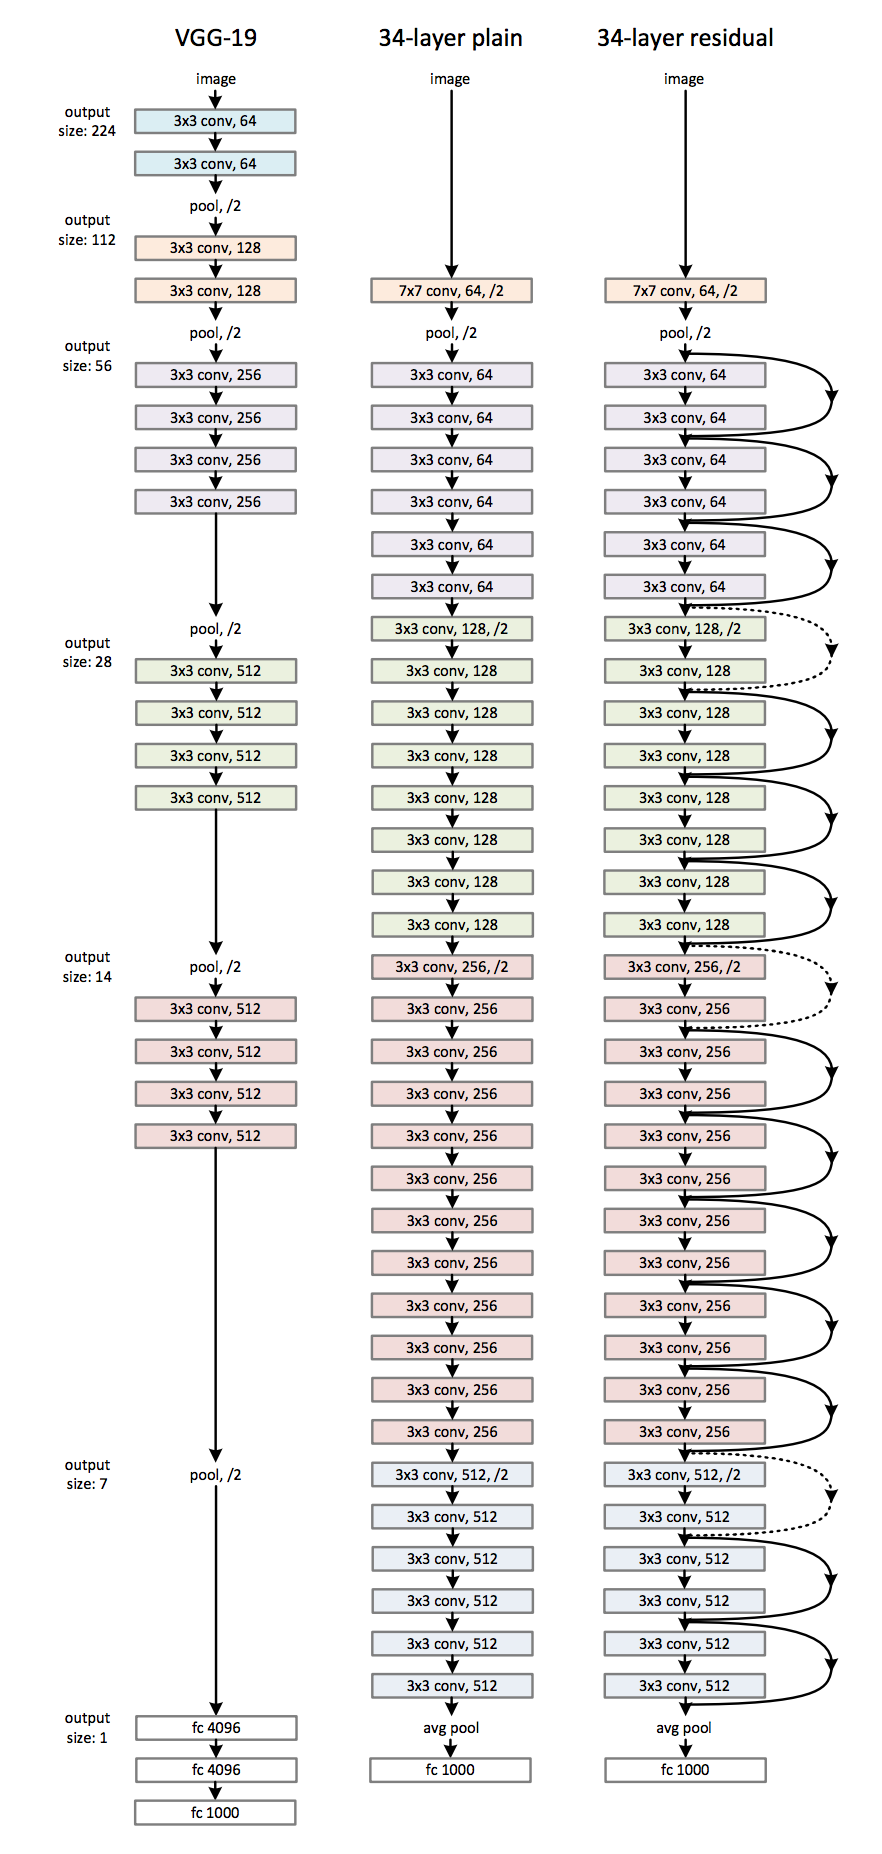
\includegraphics[scale=0.7]{figures/resnet_vgg_comparison.png}
  \centering
  \caption{A comparison of two popular CNN architectures - ResNet and VGG}
  \label{fig:vgg_resnet_comparison}
\end{figure}

\subsection{Inception v3} 
\label{se:inceptionv3_architecture}

Another mentioned CNN architecture is Inception v3. It uses the Inception module (see Figure \ref{fig:inception_module}) to increase the performance of the convolution layers in the neural network. The Inception v3 architecture is composed of Inception modules. The Inception module consists of multiple convolution blocks, each with a different kernel size. This allows the Inception module to gather multiple layers of abstraction in each module. The performance of ResNet-50 and Inception v3 is similar and after testing both it showed in Section \ref{se:resnet_vs_inception} that  ResNet-50 provided better results by a slight margin on this task.

\begin{figure}
  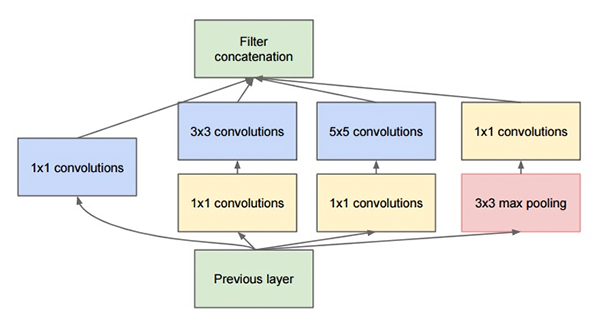
\includegraphics[scale=0.7]{figures/inception_module.png}
  \centering
  \caption{Inception v3's Inception module}
  \label{fig:inception_module}
\end{figure}


\subsection{Pretrained parameters}
\label{se:pretrained_parameters}
As seen in Figure \ref{fig:filter}, each convolution layer learns a specific level of abstraction. Those abstractions are general building blocks of images (boxes, circles, edges, etc.). This implies that if you train a CNN on one set of images, the parameters in the front convolution layers can be reused on a different task. Using this, higher accuracy can be achieved when working on small datasets. This is called pretraining or fine-tuning the model.

One of the biggest annotated image databases is ImageNet \citep{imagenet} and is the go to dataset for image classification research. Almost every modern CNN architecture was evaluated and trained on it. Downloading the parameters from those trained neural networks and initialising the model with them gives us state-of-the-art performance even on small datasets. The only needed step is to fine-tune the neural network by training it on our dataset after it was initialised with the pretrained values - called fine tuning.

Below is the Keras code for creating a pretrained model from the ImageNet dataset. First, the pretrained model is loaded without the top layer (the top layer is not important as it is a fully-connected layer which was built for 1000 classes, the convolution layers are only needed for this task). The second step is to create a small feed-forward network and append it to the end of the network. Set the pretrained convolution layers to not train and compile to model. The final softmax layer has 15 neurons as the model was tested on a dataset of 15 classes that is 2GB in size. The model was trained with Backpropagation using the Adam optimizer \citep{kingma_adam:_2014}.

\begin{lstlisting}[language=Python, caption=Creating a custom pretrained ResNet using the weights from the ImageNet dataset]

from keras.applications import ResNet50

IMG_DIM = 224
INPUT_TENSOR = Input(shape=(IMG_DIM, IMG_DIM, 3))

base_model = ResNet50(input_tensor=INPUT_TENSOR, include_top=False)

for layer in base_model.layers:
    layer.trainable = False

top_model = Sequential()
top_model.add(Flatten(input_shape=base_model.output_shape[1:]))

top_model.add(Dense(32))
top_model.add(BatchNormalization())
top_model.add(Activation('relu'))

top_model.add(Dense(64))
top_model.add(BatchNormalization())
top_model.add(Activation('relu'))

top_model.add(Dense(15, activation='softmax'))


model = Model(input= base_model.input, output= top_model(base_model.output))

    
model.compile(loss='categorical_crossentropy',
              optimizer='adam',
              metrics=['accuracy'])
\end{lstlisting}

\subsection{Improving generalization}

To improve the generalization of the model, batch normalization was added after every fully-connected layer in the network (see the code example above). Also, the input images were augmented (\ref{se:data_augmentation}). The $X_{test}$ had its images only rescaled, while $X_{train}$ and $X_{validation}$ were more aggressively augmented (random zoom, horizontal flip, rescale and sheered), this is shown in detail in the Figure \ref{fig:data_augmentation}.

\begin{lstlisting}[language=Python, caption=Data augmentation of the input dataset (images)]

batch_size = 16

train_datagen = ImageDataGenerator(
        rescale=1./255,
        shear_range=0.2,
        zoom_range=0.2,
        horizontal_flip=True)

test_datagen = ImageDataGenerator(rescale=1./255)

train_generator = train_datagen.flow_from_directory(
        '../input/train',
        target_size=(150, 150),
        batch_size=batch_size,
        class_mode='categorical') 


validation_generator = test_datagen.flow_from_directory(
        '../input/validation',
        target_size=(150, 150),
        batch_size=batch_size,
        class_mode='categorical')
        
\end{lstlisting}

\chapter{Data}

Many would argue that the data is the most important part of the machine learning system \citep{deep_learning}. If the training data does not represent the real world input of the system in production (as a product) the machine learning algorithm is good as useless. Furthermore, the quantity of data is crucial for deep learning algorithms. Compared to traditional machine learning algorithms, deep learning algorithms gain more performance scale from the dataset size \citep{deep_learning}. Therefore, data collection for this problem is a crucial step in the machine learning pipeline and impacts the whole solution.

\section{ImageNet}
\label{se:imagenet}

One of the largest labeled image datasets freely opened to the public is ImageNet \citep{imagenet}. It contains more than 14 million images, detailed statistics of the dataset can be found in Table \ref{tb:imagenet_statistics}. To train the model for species recognition I have used a subset of images found on ImageNet. Using every class that represents a species in ImageNet is not doable on a single 2GB GPU (at least not in reasonable time), therefore I have manually picked 15 classes which give a good representation of the problem as a whole. The idea is to have some species that are similar to others, for example, multiple species of ladybugs while still having a wide variate of species that represent the diverse form of life (a typical example of an image from the ImageNet dataset can be seen in Figure \ref{fig:typical_imagenet_example}).

\begin{figure}
  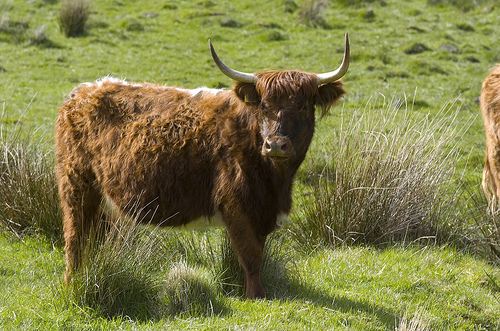
\includegraphics[scale=0.55]{figures/typical_imagenet.jpg}
  \centering
  \caption{Typical image from the ImageNet dataset, from the class herbivore}
  \label{fig:typical_imagenet_example}
\end{figure}

\begin{table}
\centering
\caption{ImageNet statistics}
\label{tb:imagenet_statistics}
\begin{tabular}{cccc}
\hline 
High level category    & synset (subcategories)    & Avg images per synset & Total images  \\ \hline
amphibian & 94 & 591 & 56K \\
animal & 3822 & 732 & 2799K \\
appliance & 51 & 1164 & 59K \\
bird & 856 & 949 & 812K \\
covering & 946 & 819 & 774K \\
device & 2385 & 675 & 1610K \\
fabric & 262 & 690 & 181K \\
fish & 566 & 494 & 280K \\
flower & 462 & 735 & 339K \\
food & 1495 & 670 & 1001K \\
fruit & 309 & 607 & 188K \\
fungus & 303 & 453 & 137K \\
furniture & 187 & 1043 & 195K \\
geological formation & 151 & 838 & 127K \\
invertebrate & 728 & 573 & 417K \\
mammal & 1138 & 821 & 934K \\
musical instrument & 157 & 891 & 140K \\
plant & 1666 & 600 & 999K \\
reptile & 268 & 707 & 190K \\
sport & 166 & 1207 & 200K \\
structure & 1239 & 763 & 946K \\
tool & 316 & 551 & 174K \\
tree & 993 & 568 & 564K \\
utensil & 86 & 912 & 78K \\
vegetable & 176 & 764 & 135K \\
vehicle & 481 & 778 & 374K \\
person & 2035 & 468 & 952K \\
\hline 
\end{tabular} 
\end{table}


\subsection{Dataset}
\label{se:dataset}

As mentioned in the previous section, the dataset - $X$ - consists of 15 species of images from the ImageNet dataset. Each species has a different number of samples, the distribution of $X_{train}$ can be seen in detail in Figure \ref{fig:training_set_class_distributon}. We can see that some classes (Mexican bean beetle and Black-footed albatross) have below an average number of images, this will yield a lower classification performance for these classes. Also, we can except the classifier to work best for the classes with above average number of images like the Ice bear species. A deeper analysis on classification performance for certain classes will be shown in further sections (Figure \ref{fig:species_confusion_matrix}).

The convolutional network accepts only a fixed size input, therefore every image in the dataset - $X$ - has to be scaled to a fixed size. Lowering the dimensions of the input image will result in a performance decrease. Therefore, after experimenting with the hyperparameter I have picked $224 \times 224$ image dimensions in order to have the optimal classification and speed performance (this dimension is also the input dimension used by the original ResNet which made preprocessing faster).

\begin{figure}
  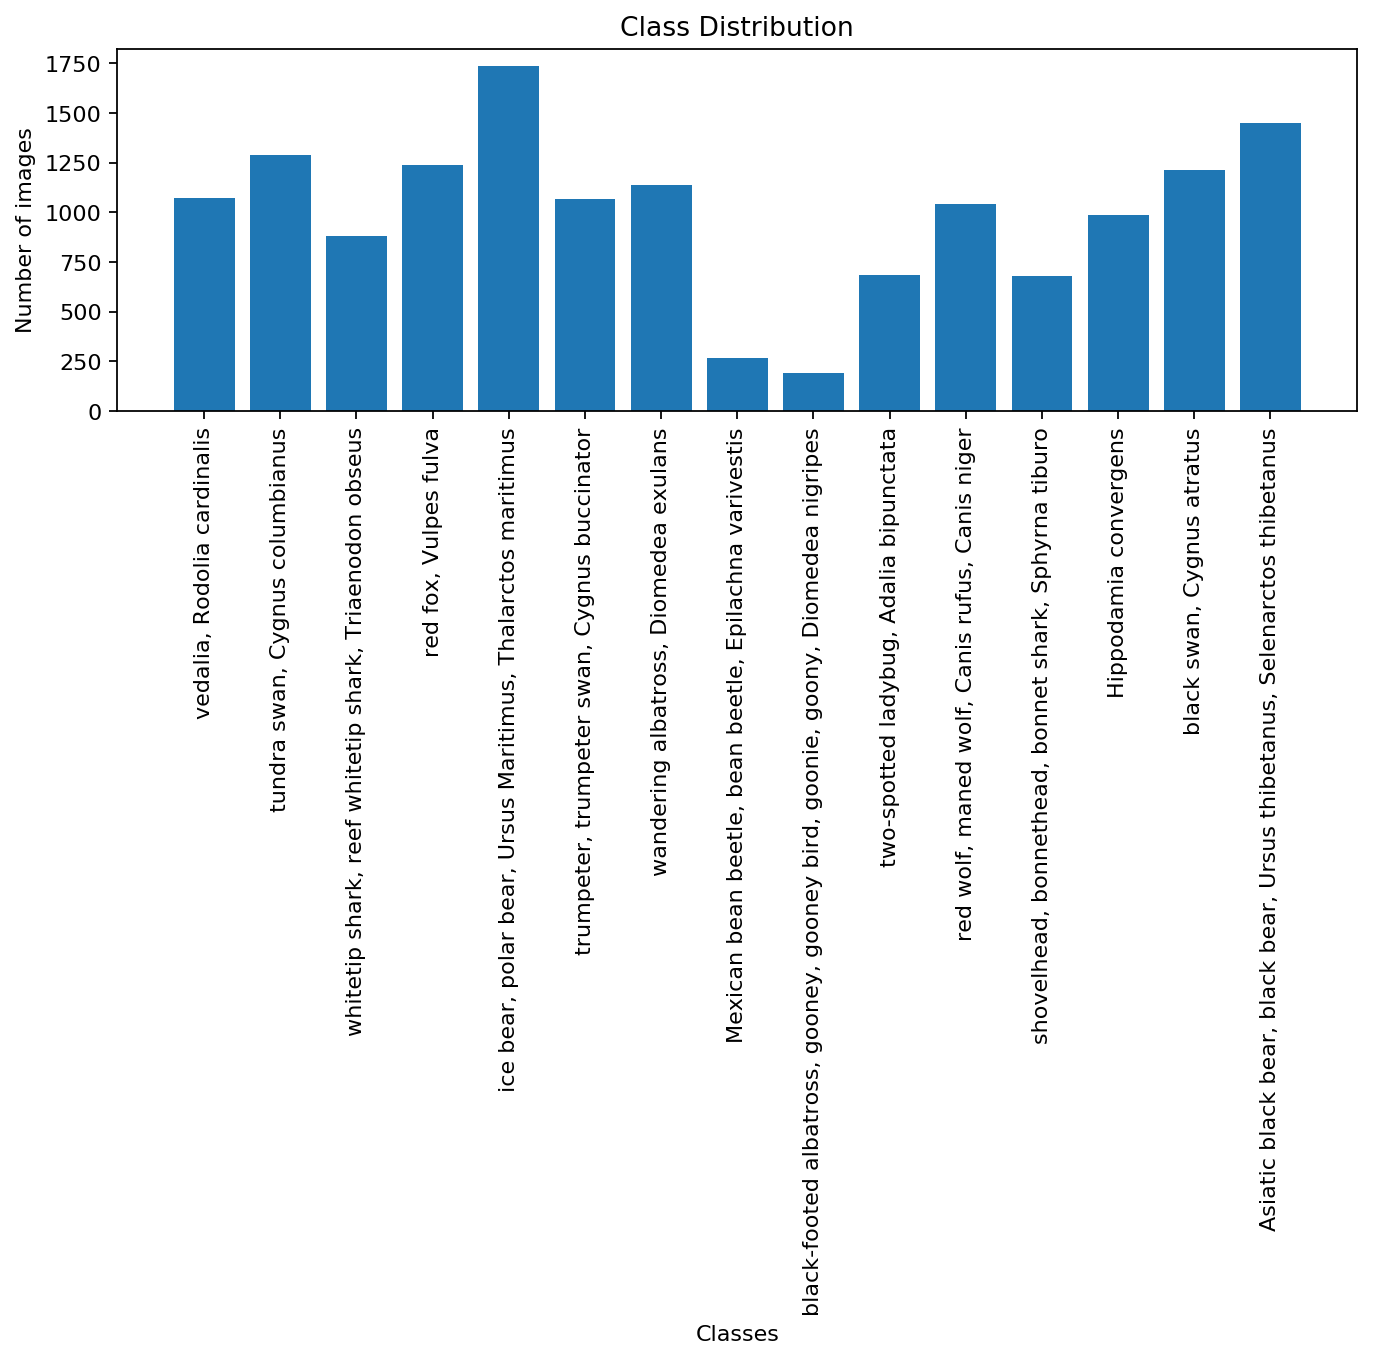
\includegraphics[scale=0.75]{figures/class_distribution.png}
  \centering
  \caption{Class distribution of training data}
  \label{fig:training_set_class_distributon}
\end{figure}


\begin{table}
\centering
\caption{Dataset statistics}
\label{tb:dataset_statistics}
\begin{tabular}{cc}
\hline 
Size [GB] & 1.6 \\ \hline 
Class number & 15 \\ 
Type & RGB Images \\ 
Train size & 14929 \\
Validation size & 1649 \\
\hline 
\end{tabular} 
\end{table}

\subsection{Preprocessing}
Preprocessing of data is an essential part of the machine learning pipeline. As state in the previous Section \ref{se:dataset}, every image has to be a fixed size in order to be able to serve as an input into the deep learning model. When scaling images to a fixed size sometimes because of the aspect ration of the image, we need to fill a part of the image with a constant pixel value.


Also, another important part of the preprocessing is the generation of the validation dataset. For the validation to be efficient the validation dataset has to represent the training dataset. Keeping that in mind, the validation set - $X_{validation}$ - was created by taking 10\% of images form each class (species).


\section{Species}
\label{se:species}

This chapter shows typical images found in the ImageNet dataset that was used as input for the model. The list of all 15 species used for model training is found in Table \ref{tb:species_list}.

\begin{table}
\centering
\caption{List of all 15 species used to train the model}
\label{tb:species_list}
\begin{tabular}{cc}
\hline 
Species (common name) & Species (Latin name)\\ \hline 
whitetip shark, reef whitetip shark & Triaenodon obseus \\
shovelhead, bonnethead, bonnet shark & Sphyrna tiburo \\
tundra swan & Cygnus columbianus \\
trumpeter, trumpeter swan & Cygnus buccinator \\
black swan & Cygnus atratus \\
wandering albatross & Diomedea exulans \\
black-footed albatross, gooney, goonie, goony & Diomedea nigripes \\
red wolf, maned wolf & Canis rufus, Canis niger \\
red fox & Vulpes fulva \\
Asiatic black bear, black bear & Ursus thibetanus\\
ice bear, polar bear & Ursus Maritimus \\
two-spotted ladybug & Adalia bipunctata \\
Mexican bean beetle, bean beetle & Epilachna varivestis \\
convergent lady beetle & Hippodamia convergens \\
vedalia & Rodolia cardinalis \\
\hline 
\end{tabular} 
\end{table}

Some of the species are shown in Figure \ref{fig:specis_image_examples}. Some species seem so similar that expert knowledge is needed (see Figures \ref{fig:adalia_bipunctata} and \ref{fig:rodolia_cardinalis}). These images can seem almost identical to an untrained eye while still being different species, or in some cases not even close in the evolutionary tree. Neural networks with enough capacity have the ability to distinguish these traits on a level that is hard to interpret.

There is a lot of noise in the images found in $X$, animals are usually found in their habitats which makes them hard to be distinguished from their surroundings. This can be seen in Figure \ref{fig:canis_rufus}, the Canis rufus is hidden and hard to see because of the color of his fur in regard to his surrounding. Or in Figure \ref{fig:sphyrna_tiburo} which has humans in the image.



\begin{figure}
    \begin{subfigure}[b]{0.32\textwidth}
        \centering
        \resizebox{\linewidth}{!}{
  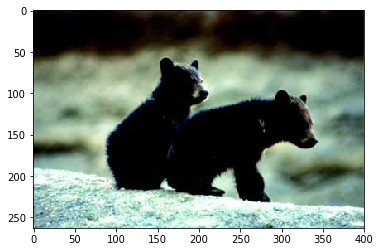
\includegraphics[scale=0.36]{figures/asiatic_black_bear.png}
        }
        \caption{Ursus thibetanus}
        \label{fig:ursus_thibetanus}
    \end{subfigure}
        \begin{subfigure}[b]{0.32\textwidth}
        \centering
        \resizebox{\linewidth}{!}{
  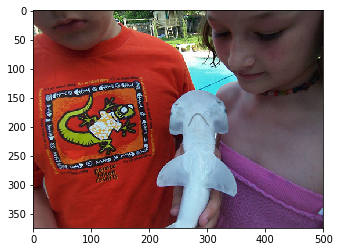
\includegraphics[scale=0.36]{figures/bonnet_shark.png}
        }
        \caption{Sphyrna tiburo}
        \label{fig:sphyrna_tiburo}
    \end{subfigure}
        \begin{subfigure}[b]{0.32\textwidth}
        \centering
        \resizebox{\linewidth}{!}{
  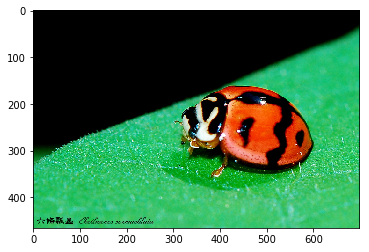
\includegraphics[scale=0.36]{figures/hippodamia_convergens.png}
        }
        \caption{Hippodamia convergens}
        \label{fig:hippodamia_convergens}
    \end{subfigure}
    
        \begin{subfigure}[b]{0.32\textwidth}
        \centering
        \resizebox{\linewidth}{!}{
  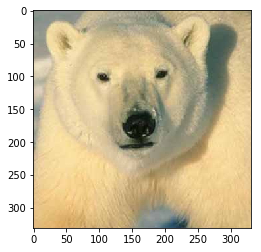
\includegraphics[scale=0.36]{figures/polar_bear.png}
        }
        \caption{Ursus maritimus}
        \label{fig:ursus_maritimus}
    \end{subfigure}
        \begin{subfigure}[b]{0.32\textwidth}
        \centering
        \resizebox{\linewidth}{!}{
  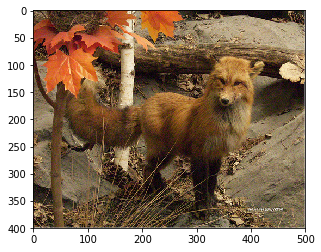
\includegraphics[scale=0.36]{figures/red_fox.png}
        }
        \caption{Vulpes fulva}
        \label{fig:vulpes_fulva}
    \end{subfigure}
        \begin{subfigure}[b]{0.32\textwidth}
        \centering
        \resizebox{\linewidth}{!}{
  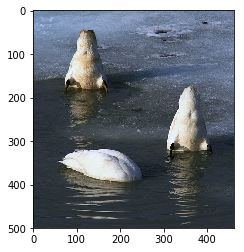
\includegraphics[scale=0.36]{figures/trumepeter_swan.png}
        }
        \caption{Cygnus buccinator}
        \label{fig:cygnus_buccinator}
    \end{subfigure}
    
     \begin{subfigure}[b]{0.32\textwidth}
        \centering
        \resizebox{\linewidth}{!}{
  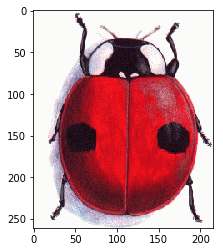
\includegraphics[scale=0.36]{figures/two_spotted_ladybug.png}
        }
        \caption{Adalia bipunctata}
        \label{fig:adalia_bipunctata}
    \end{subfigure}
        \begin{subfigure}[b]{0.32\textwidth}
        \centering
        \resizebox{\linewidth}{!}{
  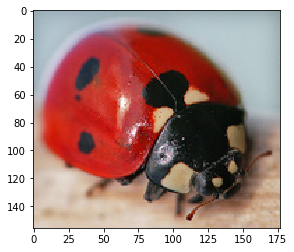
\includegraphics[scale=0.36]{figures/vedalia.png}
        }
        \caption{Rodolia cardinalis}
        \label{fig:rodolia_cardinalis}
    \end{subfigure}
        \begin{subfigure}[b]{0.32\textwidth}
        \centering
        \resizebox{\linewidth}{!}{
  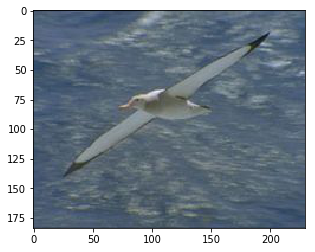
\includegraphics[scale=0.36]{figures/wandering_albatross.png}
        }
        \caption{Diomedea exulans}
        \label{fig:diomedea_exulans}
    \end{subfigure}
    
    
     \begin{subfigure}[b]{0.32\textwidth}
        \centering
        \resizebox{\linewidth}{!}{
  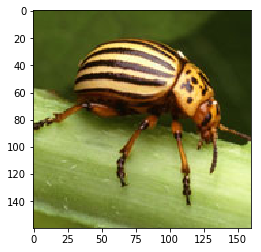
\includegraphics[scale=0.36]{figures/mexican_bean_beetle.png}
        }
        \caption{Epilachna varivestis}
        \label{fig:epilachna_varivestis}
    \end{subfigure}
        \begin{subfigure}[b]{0.32\textwidth}
        \centering
        \resizebox{\linewidth}{!}{
  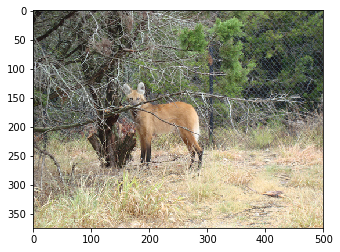
\includegraphics[scale=0.36]{figures/red_wolf.png}
        }
        \caption{Canis rufus}
        \label{fig:canis_rufus}
    \end{subfigure}
        \begin{subfigure}[b]{0.32\textwidth}
        \centering
        \resizebox{\linewidth}{!}{
  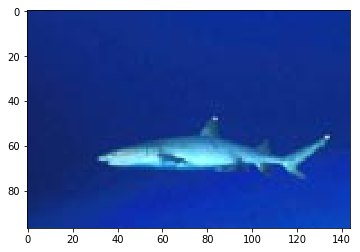
\includegraphics[scale=0.36]{figures/whitetip_shark.png}
        }
        \caption{Triaenodon obseus}
        \label{fig:triaenodon_obseus}
    \end{subfigure}
    
\caption{Examples of species with a randomly picked image from the input dataset} 
\label{fig:specis_image_examples}
\end{figure}



\chapter{Results}
\label{se:results}

\section{Hardware and software}
The model is implemented in Keras 2.0 4 \citep{keras} with Python 3.5. All the results were computed on my personal laptop with the following hardware and software specifications (Tables \ref{tb:hardware_specifications} and \ref{tb:software_specifications}). All the software was chosen to support the given hardware specifications and to be able to efficiently build and train a deep learning model, explained in detail in Section \ref{se:model}. Python is currently the leading language for deep learning, as well as TensorFlow \citep{tensorflow} and its higher-level API Keras \citep{keras}. All the programs were ran inside Docker \citep{docker} containers specifically made for the previously mentioned technology stack.

\begin{table}
\centering
\caption{Hardware specifications}
\label{tb:hardware_specifications}
\begin{tabular}{cc}
\hline 
Hardware component & Specification \\ \hline 
RAM & 8GB DDR3 \\ 
Dedicated GPU & Nvidia GTX 650m \\ 
Processor & Intel Core i7-3632QM 2.2GHz\texttt{\textbackslash}Turbo Boost 3.2GHz\\
Cuda cores & 384 \\
GPU Memory Bandwidth & 80.0 GB/sec\\
Graphics Clock & Up to 900 MHz \\
Memory Interface & DDR3\texttt{\textbackslash}GDDR5 \\
\hline 
\end{tabular} 
\end{table}

\begin{table}
\centering
\caption{Software specifications}
\label{tb:software_specifications}
\begin{tabular}{cc}
\hline 
Software & Version \\ \hline 
Operating System & Ubuntu 16.04 LTS \\ 
Python & 64-bit version 3.5 \\ 
Keras & 2.0.4 \\
TensorFlow & 1.1 \\
\hline 
\end{tabular} 
\end{table}

\section{ResNet-50 and Inception v3 comparison}
\label{se:resnet_vs_inception}

After deciding that ResNet-50 and Inception v3 were the best base CNN architectures for this task (Section \ref{se:architecture}), testing was done to decide which one performed better. ResNet-50 had the better performance and was used as the final model, all the performance metrics are shown below (Table \ref{tb:resnet_vs_inceptionv3})

\begin{table}
\centering
\caption{ResNet-50 and Inception v3 architecture comparison on the validation set}
\label{tb:resnet_vs_inceptionv3}
\begin{tabular}{ccc}
\hline 
Metric & ResNet-50 & Inception v3 \\ \hline 
Accuracy & 0.830200 & 0.81807 \\ 
Precision & 0.80108 & 0.77996 \\ 
Recall & 0.80400 & 0.78006 \\
F1 & 0.80100 &  0.77810 \\
\hline 
\end{tabular} 
\end{table}

The detailed training and validation loss and accuracy can be found in Figures \ref{fig:resnet_performance} and \ref{fig:inceptionv3_performance}. The Figures clearly show that ResNet-50 has a lower loss and higher accuracy on unseen data (validation set).

\begin{figure}
  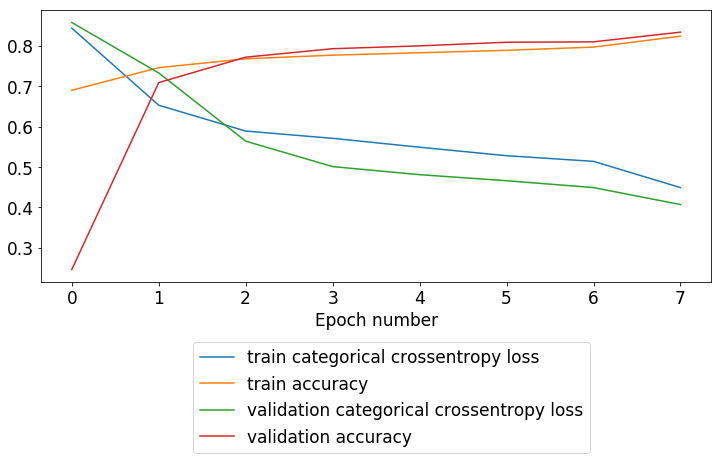
\includegraphics[scale=0.61]{figures/resnet_performance.png}
  \centering
  \caption{ResNet-50 performance on the training and the validation sets}
  \label{fig:resnet_performance}
\end{figure}

\begin{figure}
  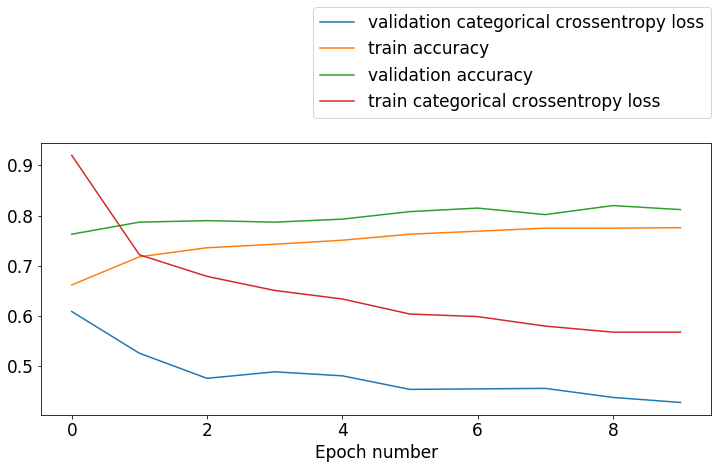
\includegraphics[scale=0.61]{figures/inceptionv3_performance.png}
  \centering
  \caption{Inception v3 performance on the training and the validation sets}
  \label{fig:inceptionv3_performance}
\end{figure}


\begin{table}
\centering
\caption{Software specifications}
\label{tb:software_specifications}
\begin{tabular}{cc}
\hline 
Software & Version \\ \hline 
Operating System & Ubuntu 16.04 LTS \\ 
Python & 64-bit version 3.5 \\ 
Keras & 2.0.4 \\
TensorFlow & 1.1 \\
\hline 
\end{tabular} 
\end{table}

\section{Performance}

In this section, different metrics and their impact on the performance of the model, as well as a detailed insight into the performance of the model is shown. The model is evaluated on a validation dataset that is created from 10\% images of every class from the whole input dataset. The distribution of the data with more information can be find the Chapter \ref{se:data}.

Classification performance is shown in Table \ref{tb:classifier_performance} with metrics described in detail in section \ref{se:metrics}. This Table shows a detailed outline of the overall classification performance of the model, but it fails to give insight into the classification performance on a class by class level. To resolve this problem, a confusion matrix is shown in Figure \ref{fig:species_confusion_matrix}. The confusion matrix shows that certain species are less likely to be confused with certain other species. The confusion matrix has a couple of clusters, the clusters appear to form near similar looking species. All the images of ladybug species look almost the same and it is natural to expect the classifier to have a worst performance with these species, a potential method for increasing the performance for these species is giving the Section \ref{se:future_work}.

This algorithm is designed to be able to scale to thousands of species. To do so it must keep its accuracy even with different subsets of the original input dataset. To test this, the model was evaluated for different subsets of species - the result is shown in Figure \ref{fig:model_acc_class_num}. The accuracy falls and raises for lower class numbers meaning that the model works well but the number of images per class has the biggest effect on the model performance. Building an ingestion platform for data collection, for example with web scraping, would significantly increase the performance of the model as most of the classes have around 1000 images which is considered relatively small for deep learning models. 

The quality of the dataset is also crucial for the model's performance as images that do not represent the class will lower the performance and make the training phase difficult. Collecting images that represent a class is difficult, collecting high-quality images is even more difficult. Big companies usually have team's that annotate and collect data for machine learning algorithms and products.

\begin{table}
\centering
\caption{Classifier performance}
\label{tb:classifier_performance}
\begin{tabular}{cc}
\hline 
Metrics & Value \\ \hline 
Accuracy &  0.83505\\ 
Precision & 0.80856 \\ 
Recall & 0.80211 \\
F1 & 0.80311 \\
\hline 
\end{tabular} 
\end{table}

\begin{figure}
  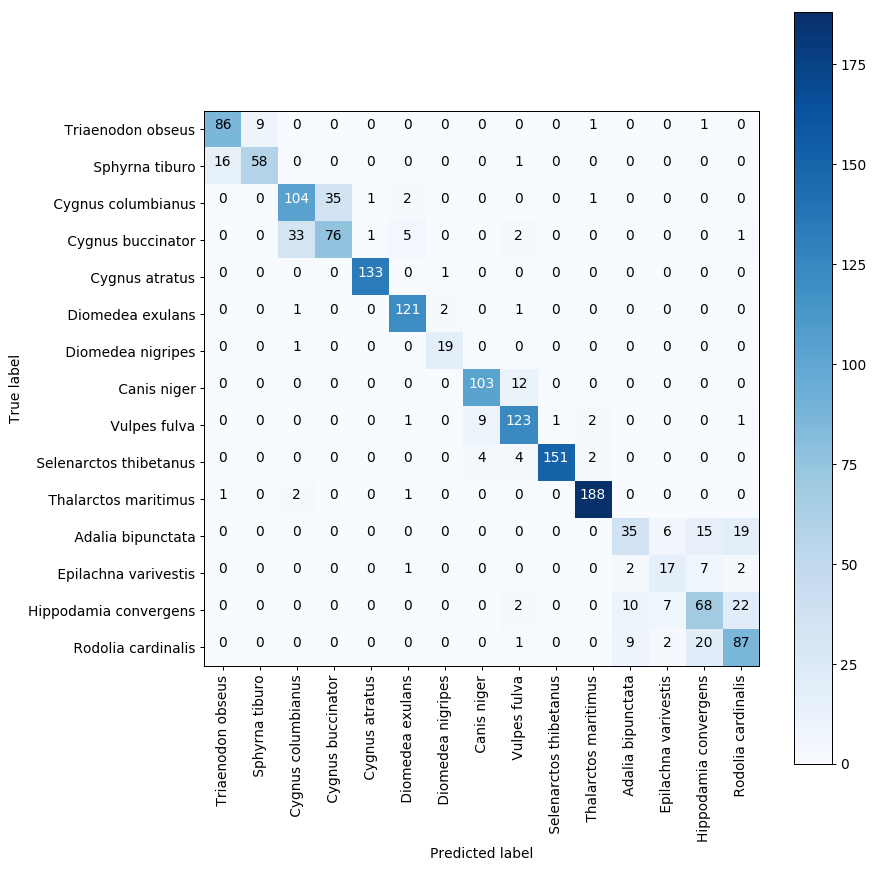
\includegraphics[scale=0.66]{figures/confusion_matrix.png}
  \centering
  \caption{Confusion matrix generated on $X_{validation}$}
  \label{fig:species_confusion_matrix}
\end{figure}

\begin{figure}
  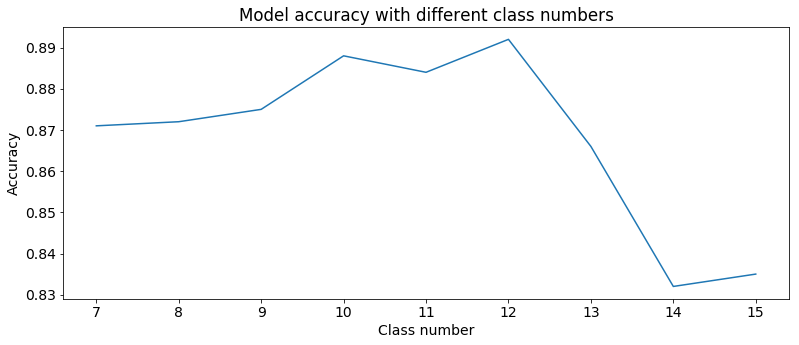
\includegraphics[scale=0.59]{figures/model_acc_class_num.png}
  \centering
  \caption{Model accuracy compared with different number of classes in $X_{validation}$ using the final model}
  \label{fig:model_acc_class_num}
\end{figure}


\section{Memory footprint}

Using a pretrained model allows for faster training as the only parameters that change are the one's int the last layer of the network. A number of trainable and non-trainable parameters can be found in Table \ref{tb:model_params}.

Each parameter is a neuron's connection weight - 32-bit float number. Trainable parameters need additional memory because each parameter has to have a gradient calculated for it (Backpropagation). Additionally some layers require more parameters, such as Batch normalization. 

\begin{table}
\centering
\caption{Number of parameters}
\label{tb:model_params}
\begin{tabular}{cc}
\hline 
Parameter type & Number \\ \hline 
Trainable &   1,321,487\\ 
Non-trainable & 53,120 \\ 
Total & 23,589,760 \\
\hline 
\end{tabular} 
\end{table}

\section{Future work}
\label{se:future_work}

Firstly, getting better hardware and scaling the model to more than a thousand species is crucial for a reasonable product. Currently, results give the information that the model is scalable and that the current performance is impacted mostly by species that look similar. 

Increasing the number of annotated images per species would also greatly increase the performance of the model. This is true especially for the species with below average number of images (Figure \ref{fig:training_set_class_distributon})

The confusion matrix is able to give insight into which classes confuse the model. Using this information an algorithm can be made that combats those deficiencies. For example, building separate classifiers for each cluster in confusion matrix could yield better model performance. This is called a hierarchical convolution neural network (HD-CNN) and is a topic that is currently being researched \citep{yan_hd-cnn:_2015, yan_hd-cnn:_2015-1}. 

\chapter{Conclusion}
With the increase in high quality annotated data, and both, hardware and software improvements - deep learning model's will only get better. Also, with the abundance of high-level deep learning framework, the barrier to enter in the deep learning field is lower each day. This will with time spur, even more, innovation and progress in the field. This can be seen already today - with new models, architectures, techniques being developed on a monthly basis.

Keeping up with the pace of deep learning research is crucial as using and exploring new techniques usually yields the most competitive model performance. Also, with the increase of new techniques, a framework for rapid iteration and exploring is necessary for the development of competitive performance models. Therefore, using Keras and similar frameworks allows for a significant improvement in performance.

Using modern deep learning techniques can provide great results on difficult tasks - such as image-based species classification.

This model still has a lot of ways to improve. Firstly, it should be able to classify more species and also be able to work in difficult terrain where an internet connection is not reliable. Therefore, an embedded version of the algorithm should be developed for such a scenario. This means that the whole model should be able to run on a mobile device.


\bibliographystyle{fer}
\bibliography{master_thesis}


\hrvtitle{Filogenetska klasifikacija vrsta}
\begin{sazetak}
U ovom radu dajem svoje rješenje za filogenetsku klasifikaciju vrsta. Napravio sam algoritam baziran na strojnom učenju. Algoritam je implementiran u programskom jeziku Python uz korištenje modernih biblioteka i radnih okvira. Program se koristi za klasifikaciju vrsta iz slika.
 

\kljucnerijeci{Filogenetika, Strojno učenje, Klasifikacija}
\end{sazetak}

% TODO: Navedite naslov na engleskom jeziku.
\engtitle{Image Based Phylogenetic classification}
\begin{abstract}
The goal of this thesis is to study the problem of phylogenetic classification based on image data. The work will entail a survey of recent related literature, algorithm development based on machine learning, and the implementation in the Python programming language using existing frameworks. The solution will be applied to the collection of publicly available images.

\keywords{
Phylogenetics, Machine learning, Classification}
\end{abstract}

\end{document}
